\documentclass[a4paper, 11pt, oneside]{report} 
\usepackage[utf8]{inputenc}
\usepackage[dutch]{babel}
\usepackage{amsmath}
\usepackage{amsfonts}
\usepackage{amssymb}
\usepackage{graphicx}
\usepackage{caption}
\usepackage[table,xcdraw]{xcolor}
\usepackage[toc,page]{appendix}
\usepackage{hyperref}
\usepackage{titlesec}
\usepackage{listings}
\usepackage{float}
\usepackage{tikz}
\usetikzlibrary{trees}
\usepackage{tikz-qtree}
\usepackage{graphicx}
\usepackage{fancyref}
\usepackage{wrapfig}
\usepackage{url}
\usepackage{pdflscape}
\usepackage{fancyvrb}
\usepackage{fancyhdr}
\usepackage{subfig}
\usepackage{tabularx}
\usepackage{apacite}
\usepackage{longtable}
\usepackage{titlecaps}
%\usepackage[T1]{fontenc}
\usepackage{titlesec, blindtext, color}
\definecolor{gray75}{gray}{0.75}
\newcommand{\hsp}{\hspace{20pt}}
\usepackage{pdfpages}
\usepackage{afterpage}
\usepackage{siunitx}

\newcolumntype{L}[1]{>{\raggedright\arraybackslash}p{#1}}

\titleformat{\chapter}[hang]{\huge\bfseries}{\thechapter\hsp\textcolor{gray75}{|}\hsp}{0pt}{\Large\bfseries}

\def\figureautorefname{Figuur}
\def\sectionautorefname{Paragraaf}
\def\chapterautorefname{Hoofdstuk}
\def\tableautorefname{Tabel}
\def\equationautorefname{Vergelijking}
\DeclareRobustCommand{\VAN}[3]{#2} % set up for citation

\lstset { %
	language=C++,
	backgroundcolor=\color{black!3}, % set backgroundcolor
	basicstyle=\footnotesize,% basic font setting
}

%% Sets page size and margins 
\usepackage[a4paper,top=3cm,bottom=3cm,left=3cm,right=3cm,marginparwidth=1.75cm]{geometry}

\author{M.W.J. Berentsen}
\font\myfont=cmr12 at 40pt
\title{\myfont Drone meshnetwerk simulatie}
\usepackage{titling}

\newcommand{\subtitle}[9]{%
	\posttitle{%
		\par\end{center}
	\begin{center}\large#1\end{center}
	\begin{center}\large#2\end{center}
	\vskip0.5em
	\begin{center}\normalsize#3\end{center}
	\begin{center}\large#4\end{center}
	\begin{center}\large#5\end{center}
	\begin{center}\large#6\end{center}
	\begin{center}\normalsize#7\end{center}
	\begin{center}\normalsize#8\end{center}
	\begin{center}\normalsize#9\end{center}
	\vskip0.5em}%
	\rfoot{{\footnotesize \textbf{#1}}}
}

\subtitle{Software Design Document}{Versie 1.0}{Alten Nederland B.V.}{Hogeschool van Arnhem en Nijmegen}{HBO Technische Informatica - Embedded Software Developement }{MWJ.Berentsen@student.han.nl}{Studentnummer: 561399}{Docent: J. Visch, MSc}{Assessor: ir. C.G.R. van Uffelen}

\setlength{\parindent}{0pt}
\setlength{\parskip}{5pt plus 2pt minus 1pt}



\hypersetup{colorlinks=true, urlcolor=red,citecolor=black,linkcolor=blue}  % Colours hyperlinks in blue, but this can be distracting if there are many links.
\setcounter{tocdepth}{2}

\newenvironment{spmatrix}[1]
{\def\mysubscript{#1}\mathop\bgroup\begin{pmatrix}}
	{\end{pmatrix}\egroup_{\textstyle\mathstrut\mysubscript}}

\usepackage{fancyhdr}
\pagestyle{fancy}

\setlength\headheight{26pt} %% just to make warning go away. Adjust the value after looking into the warning.
% \rhead{{\color{blue}\rule{1cm}{1cm}}}

\rhead{
\includegraphics[height=1cm]{Afbeeldingen/han.png}}


\begin{document}
\begin{figure}
	\begin{center}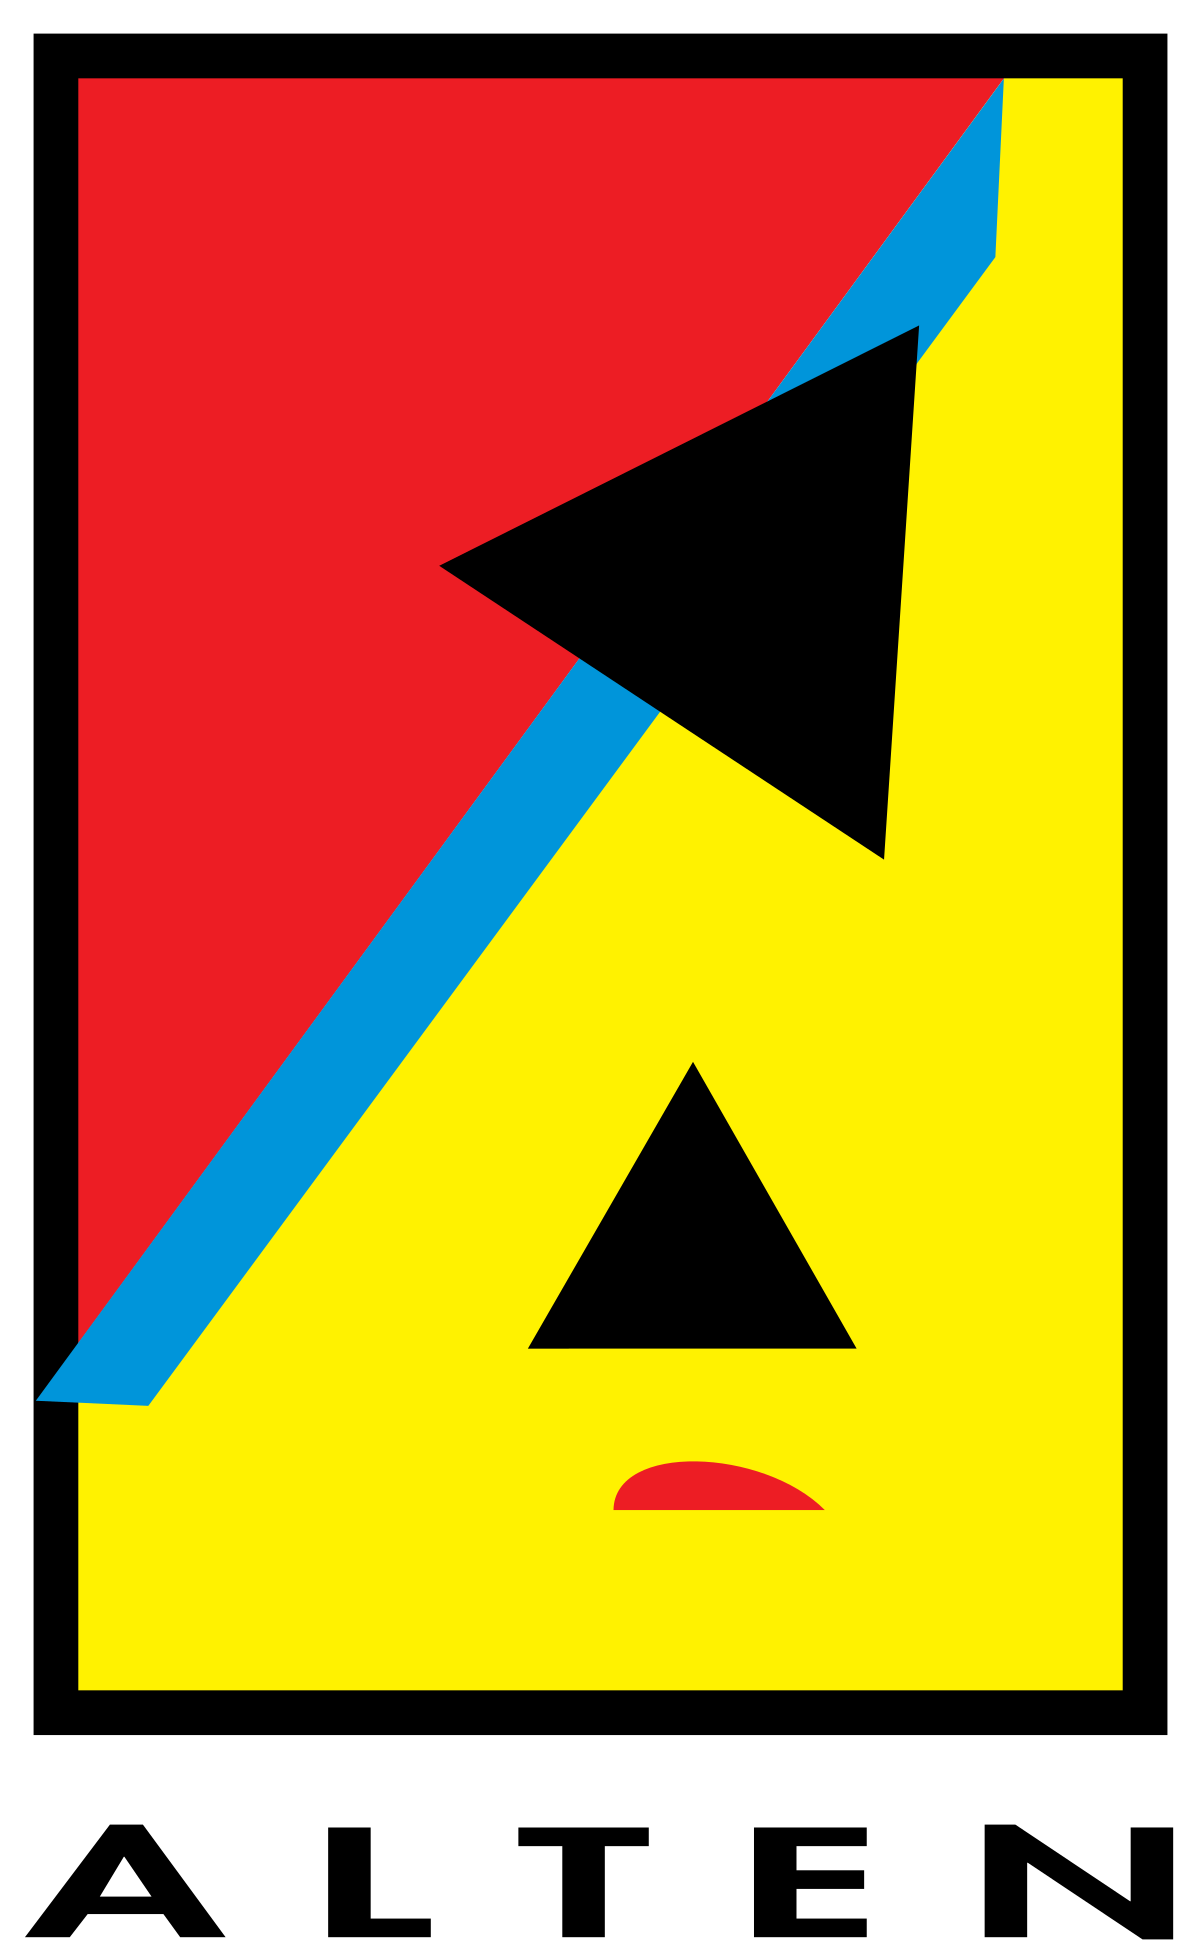
\includegraphics[scale=0.1]{Afbeeldingen/alten.png}\end{center}
\end{figure}
\maketitle

\tableofcontents
\clearpage




\chapter{Inleiding}
\label{inleiding}
Het volgende verslag betreft de Software Requirements Specification voor de afstudeerstage van Maurice Berentsen (hierna: student).
Dit document volgt het document: \textit{"Software Design Description Template"} \cite{template:sdd}

Het beschrijft de hoe de uiteindelijke applicatie eruit zal zien en wat de functionaliteit hiervan zal zijn. Op de manier is het voor de student maar ook betrokken partijen duidelijk wat er gerealiseerd zal worden. Het verduidelijk de werking van de sub-componenten en de onderlinge relaties. 

\section{Leeswijzer}
\label{inleiding:beschrijving:leeswijzer}
Eerst zal een korte beschrijving gegeven worden van het doel van dit document.Daarna wordt er door middel van een tabel een begrippenlijst toegelicht. In het tweede hoofdstuk is als eerste een component diagram te vinden waarin de functionaliteit van de verschillende componenten te vinden is en de manier waarop deze componenten met elkaar communiceren. Vervolgens is de algemene flow van het programma te zien, hierin wordt duidelijk welke stappen er onder water worden genomen als er een bepaalde actie wordt uitgevoerd. In hoofdstuk drie worden alle subsystemen duidelijk uitgewerkt en worden de ontwerpen van deze systemen uitgewerkt. 
\section{Begrippenlijst}
\label{inleiding:begrippenlijst}

% Please add the following required packages to your document preamble:
% \usepackage[table,xcdraw]{xcolor}
% If you use beamer only pass "xcolor=table" option, i.e. \documentclass[xcolor=table]{beamer}
\begin{table}[H]
\centering

\label{begrippen}
\begin{tabular}{|l|l|}
\hline
\rowcolor[HTML]{C0C0C0}
Term        & Omschrijving                                                         \\ \hline
term        & Omschrijving                                                      	\\ \hline

\end{tabular}
\caption{Begrippenlijst}
\end{table}

\chapter{Architectural Overview}
\label{architectural}
In het component diagram \autoref{fig:componentdiagram} op de volgende pagina is te zien dat bepaalde componenten voorzien zijn van een andere kleur. 
De groene kleur betekend dat het component voorzien is door gazebo.
De rode en blauw kleur zijn gegeneerd door ROS waarbij de rode een rosservice zijn en de blauwe een rostopic.
Op het hoogste niveau is het diagram te verdelen in vier groepen.

\section{Hoofdcomponenten}

\textbf{Communication} is het component die de beslissingen neemt voor de communicatie.
Het heeft de intelligentie om het netwerk in kaart te brengen en te routeren.
Daarnaast is het in staat om een beslissing te nemen om een verzoek te sturen om de drone te verplaatsen.
Tenslotte bevat het meerdere berichten die gebruikt om het netwerk te kunnen onderhouden en op te bouwen.    

\textbf{Drone} is op dit moment een leeg component waar alleen een high level interface aanwezig is die de mogelijkheid biedt om de huidige locatie van een drone terug te geven of een nieuwe locatie als doel te geven aan de drone. 

\textbf{Gazebo} is de plek waar de virtualisatie van de drone plaats vindt.
Er kunnen virtuele router of gateway drones gemaakt worden die voorzien zijn van een virtuele Raspberry Pi ingeladen met de juiste software en een virtuele drone motor.
Deze worden als model plug-in gekoppeld aan de drone in een gesimuleerde wereld waar Gazebo vervolgens physics op de drones kan uitvoeren. 

\textbf{ROS} is het component waar de simulatie van de communicatie plaats vindt.
Er is een virtuele NRF24 om te communiceren met andere nodes in het netwerk.
De aanwezige WirelessSignalSimulator zorgt dat dit realistisch gebeurd door alleen communicatie uit te voeren als dit volgens de voorwaarden mag.
Dit bepaald de simulator op basis van informatie die het krijgt van Gazebo en de NRF.
Tenslotte is er een DroneManager aanwezig die een interface aanbiedt via ros voor de ontwikkelaar om verbinding te maken met de gateways uit het netwerk.

\textbf{Raspberry Pi} is het component die zich onderscheid in twee rollen, een Raspberry Pi kan de rol van gateway hebben of de rol van router in de het meshnetwerk.

\textbf{NRF24} is het gebruikte component om draadloze communicatie mogelijk te maken. Het is voorzien van een driver in de vorm van een low level interface en bied zich aan via een high level interface voor communicatie.

Na het component diagram zal elke subcomponent kort toegelicht worden


\begin{landscape}
	\begin{figure}[p]%
		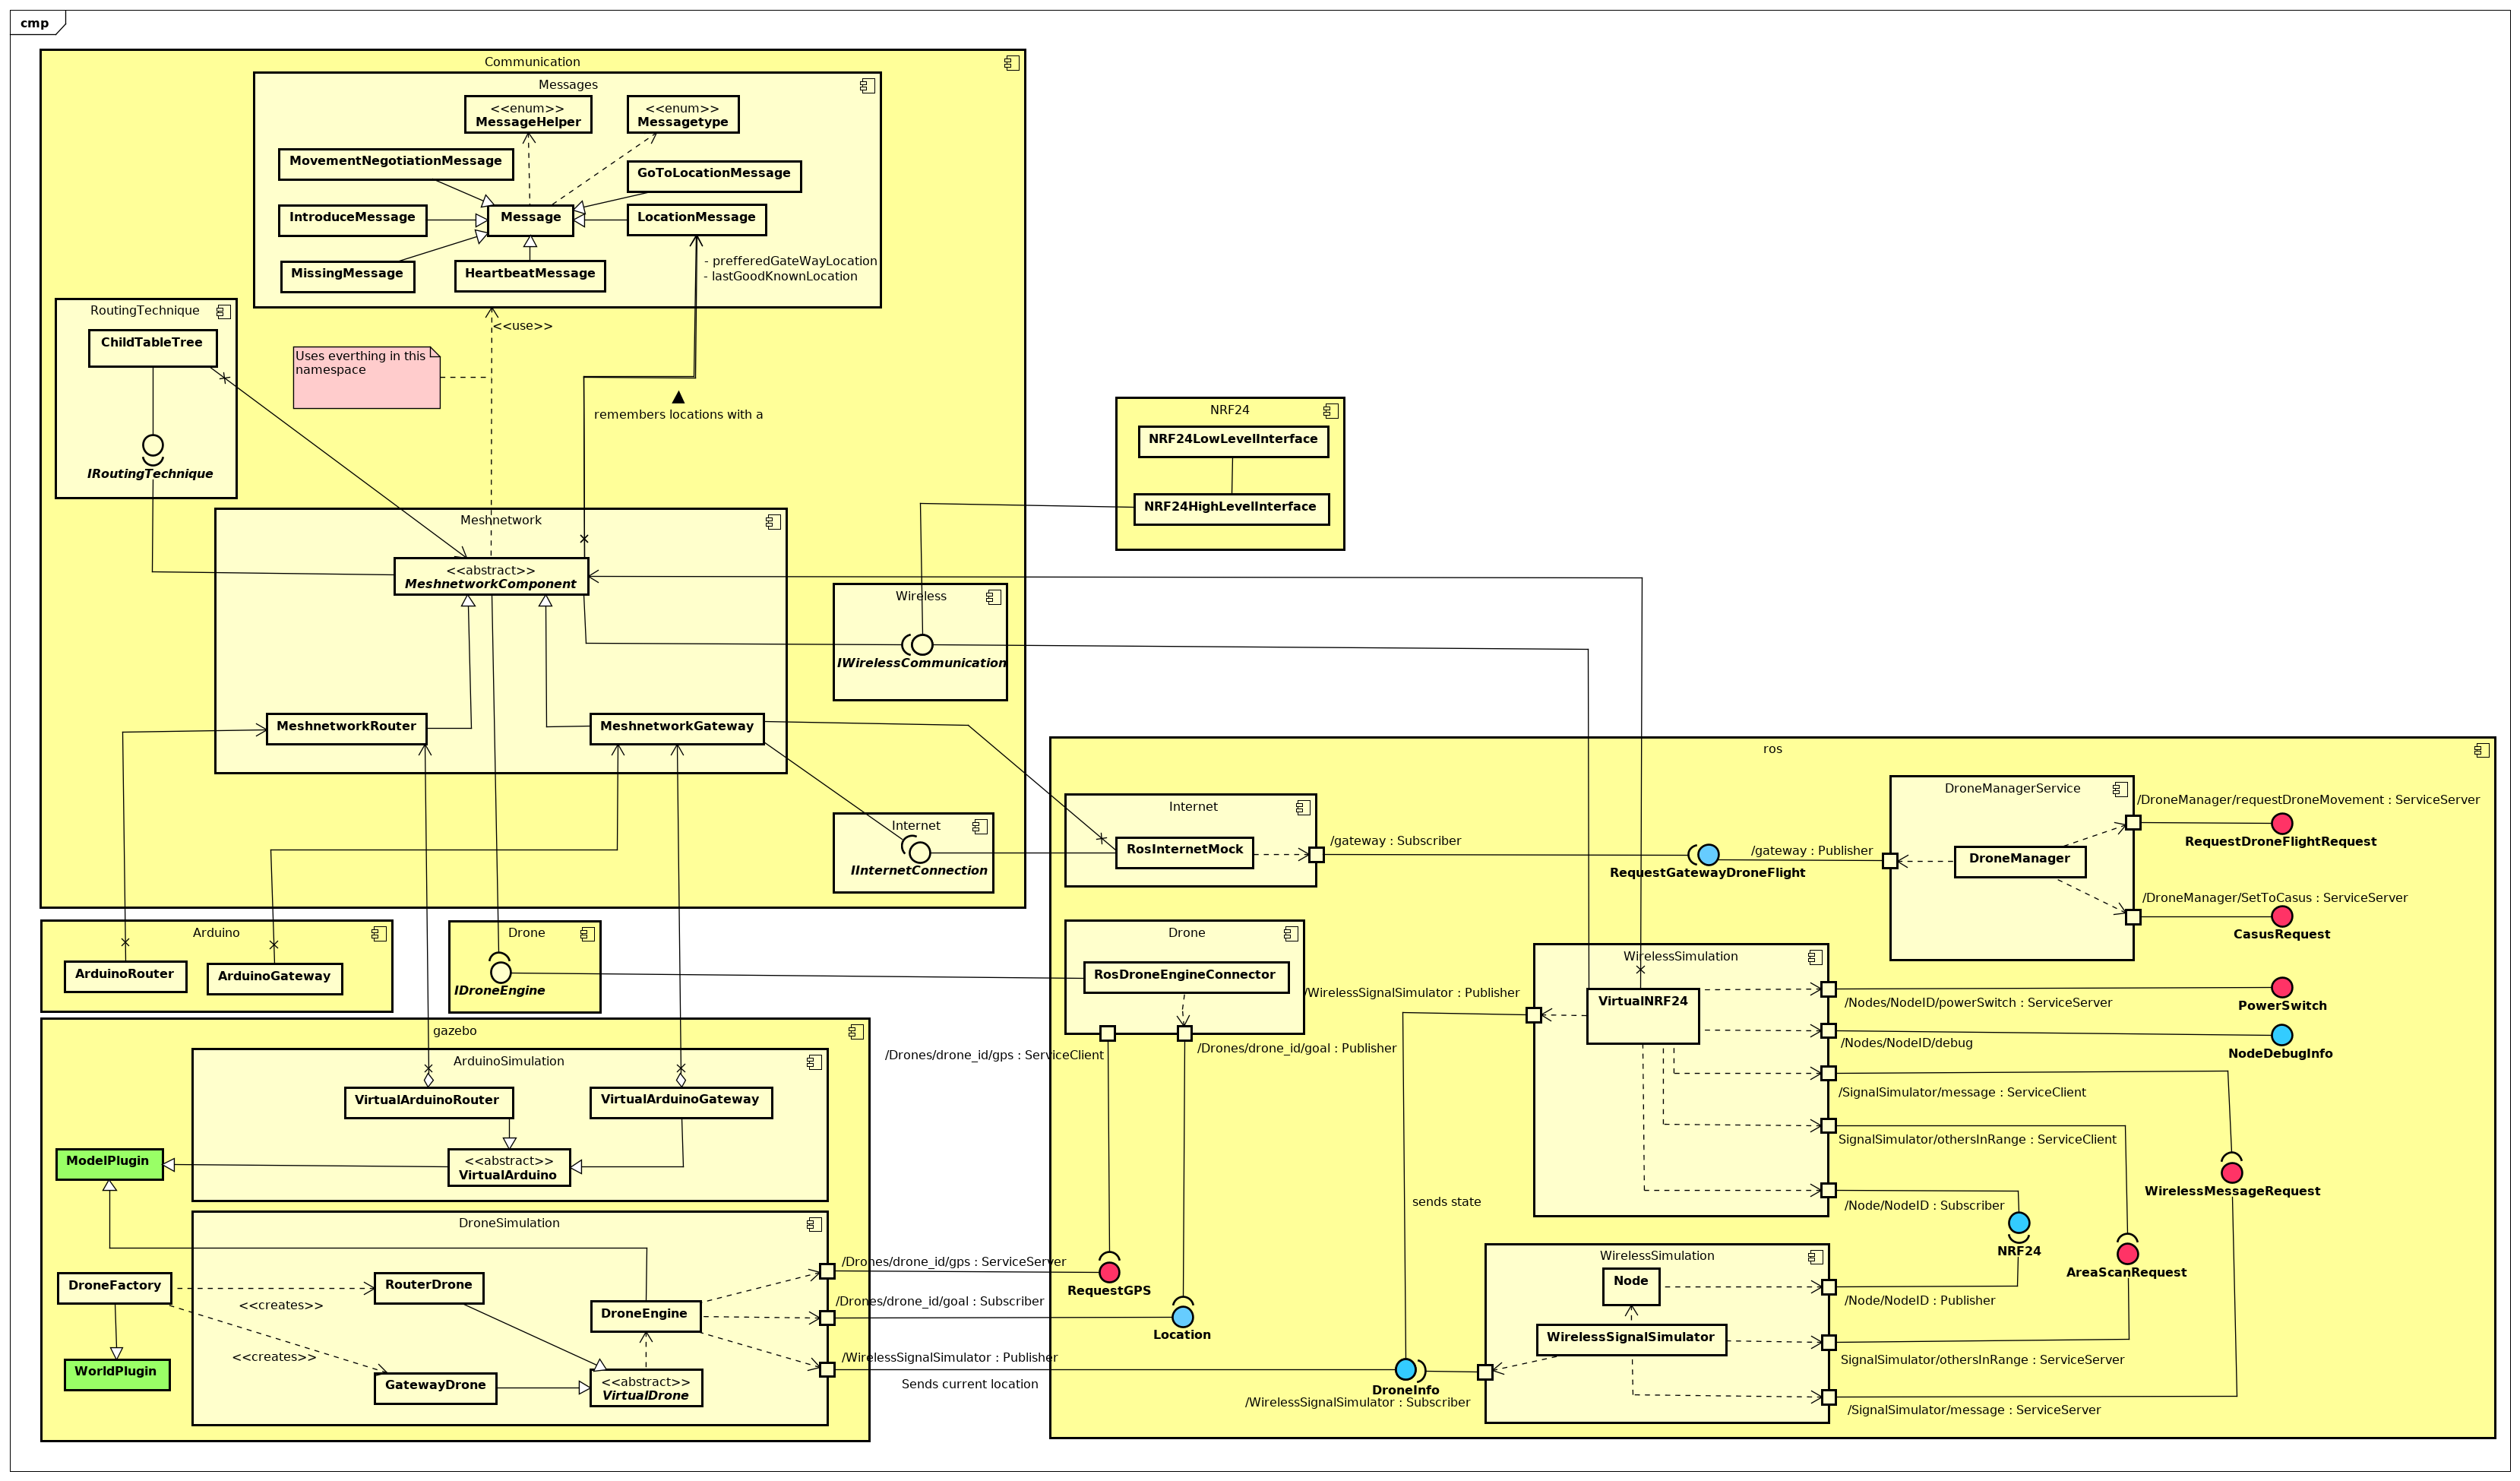
\includegraphics[width=\linewidth]{Afbeeldingen/ComponentDiagram.png}%
		\caption{Globale component diagram}
			\label{fig:componentdiagram}
	\end{figure}%
\clearpage
\end{landscape}
\clearpage


\section{Interfaces}
\label{architectural:interfaces}
\subsection{IInternetConnection}
\label{architectural:interfaces:IInternetConnection}
Deze high level interface wordt gebruikt voor het leggen van een verbinding naar een extern punt buiten het netwerk. Omdat de gateway zich alleen hoeft te verbinden met een punt bestaat deze interface alleen uit een connect en een disconnect.
\subsection{IGatewayCommands}
\label{architectural:interfaces:IGatewayCommands}
Deze interface wordt gebruikt voor het ontvangen van commando's via een verbinding met een extern punt buiten het netwerk. Op dit moment is er alleen een functie aanwezig voor het verzoeken van een drone verplaatsing
\subsection{IWirelessCommunication}
\label{architectural:interfaces:IWirelessCommunication}
In deze interface wordt de functionaliteit gesteld waar een draadloos communicatiemiddel aan moet voldoen. Het bevat functies om een antenne te starten en te stoppen. Het versturen van een bericht naar een specifiek punt of het zenden naar elke punt in de buurt. Er is een functie aanwezig om wanneer mogelijk debugging te gebruiken. Tenslotte moet een aansluitend component met deze interface moeten kunnen teruggeven of deze aan of uit staat.

\subsection{IMeshNetwork}
\label{architectural:interfaces:IMeshNetwork}
Deze interface wordt aangeboden om een aangesloten draadloos communicatie middel de mogelijkheid te geven om berichten door te kunnen geven aan het \nameref{architectural:subcomponenten:MeshnetworkComponent} en het ID van dit component kenbaar te maken.

\subsection{IMeshDebugInfo}
\label{architectural:interfaces:IMeshDebugInfo}
Deze interface wordt aangeboden om een verzameling variabelen openbaar te maken die nuttig zijn als debug informatie.

\subsection{NRF24HighLevelInterface}
\label{architectural:interfaces:NRF24HighLevelInterface}

Deze high level interface is de aangeboden interface van de NRF24 en voldoet aan de interface \nameref{architectural:interfaces:IWirelessCommunication}. Het praat direct met de driver van de NRF24.  

\subsection{NRF24LowLevelInterface}
\label{architectural:interfaces:NRF24LowLevelInterface}
Deze low level interface is de driver van de NRF24


\subsection{IDroneEngine}
\label{architectural:interfaces:IDroneEngine}
Een drone engine interface representeert de aansluiting met een drone.
Hierin moet het mogelijk zijn om een doel coördinaat te sturen naar de drone om zich naartoe te verplaatsen. 
Daarnaast moet het mogelijk zijn voor een drone om de huidige positie terug te geven.
\subsection{IRoutingTechnique}
\label{architectural:interfaces:IRoutingTechnique}
Deze interface bevat functies voor het uitvoeren van een routeringstechniek.
Het heeft functies voor het starten en onderhouden van het netwerk.
Daarnaast zijn er functies hoe gereageerd moet worden op het vinden en verliezen van andere netwerkpunten.
Er zijn functies aanwezig om een adres op te halen waar naartoe gezonden moet worden om een punt te bereiken.
Ook kan er opgehaald worden welke punten zijn aangesloten, hoeveel punten dit zijn en hoeveel directe aansluitingen er zijn.
Tenslotte is er functie aanwezig die aangeroepen wordt zodra een drone zich verplaatst zodat hier adequaat op gereageerd kan worden.

\section{Ros topics en services}
\label{architectural:ros}
Zoals al eerder benoemd wordt er gebruik gemaakt van de transportlaag van ROS. Dit wordt gedaan in de vorm van Ros topics en services. Hieronder worden de messages en services kort toegelicht.
%ROS SERVICES
\subsection{RequestGatewayDroneFlight}
\label{architectural:ros:service:RequestGatewayDroneFlight}
Via deze aangeboden service is het mogelijk om een verzoek te sturen naar de gateway voor een verplaatsing. In het verzoek moet het nodeID en locatie zitten.


\subsection{CasusRequest}
\label{architectural:ros:service:CasusRequest}
Deze service maakt het mogelijk om een casus posities door te sturen naar de drones.

\subsection{PowerSwitch}
\label{architectural:ros:service:PowerSwitch}
Via deze simpele service kan een \nameref{architectural:subcomponenten:VirtualNRF24} aan of uit gezet worden.

\subsection{WirelessMessageRequest}
\label{architectural:ros:service:WirelessMessageRequest}
De \nameref{architectural:subcomponenten:VirtualNRF24} gebruikt deze service om een NRF24 bericht te versturen naar een andere NRF24. De response geeft aan of het zenden lukte.

\subsection{AreaScanRequest}
\label{architectural:ros:service:AreaScanRequest}
Deze service kan aangeroepen worden om de id's van alle nodes binnen het bereik van een node terug te krijgen. 
Dit is nodig om een algemene zending naar iedereen binnen bereik mogelijk te maken.

\subsection{RequestGPS}
\label{architectural:ros:service:RequestGPS}
Deze service wordt aangeboden door de \nameref{architectural:subcomponenten:DroneEngine} en biedt de mogelijkheid om de huidige locatie van een drone op te vragen. 

%ROS TOPICS
\subsection{RequestGatewayDroneFlight}
\label{architectural:ros:topic:RequestGatewayDroneFlight}
Dit topic wordt gebruikt om locatieverplaatsingverzoeken op te publiceren. 

\subsection{NodeDebugInfo}
\label{architectural:ros:topic:NodeDebugInfo}
Elke \nameref{architectural:subcomponenten:VirtualNRF24} maakt wanneer dit verzocht wordt een Debug topic aan. Hierop wordt informatie gepubliceerd wat van toegevoegde waarde is voor ontwikkelaars.

\subsection{NRF24}
\label{architectural:ros:topic:NRF24}
Een \nameref{architectural:subcomponenten:VirtualNRF24} luistert naar dit topic om zo berichten te kunnen ontvangen.

\subsection{Location}
\label{architectural:ros:topic:Location}
Het location topic representeert de verbinding die een \nameref{architectural:subcomponenten:MeshnetworkComponent} zou hebben met een drone op doelen op te versturen waar de Drone heen moet vliegen. 

\subsection{DroneInfo}
\label{architectural:ros:topic:DroneInfo}
Dit topic is essentieel voor de \nameref{architectural:subcomponenten:WirelessSignalSimulator}. De informatie die hierop gepubliceerd wordt omvat informatie over de locatie van een \nameref{architectural:subcomponenten:VirtualNRF24} of die aan staat en naar welk \nameref{architectural:ros:topic:NRF24} topic deze luistert.

\chapter{Detailed Design Description}
\label{DetailedDesign}

\section{Deployment Diagram}
\label{DetailedDesign:deployment}
In dit deployment diagram staan de executables (ROS nodes) die opgestart worden door de verschillende launch files, daarnaast zijn ook de twee executables meegenomen die gebruikt worden op de Raspberry Pi's

\begin{figure}[H]
	\begin{center}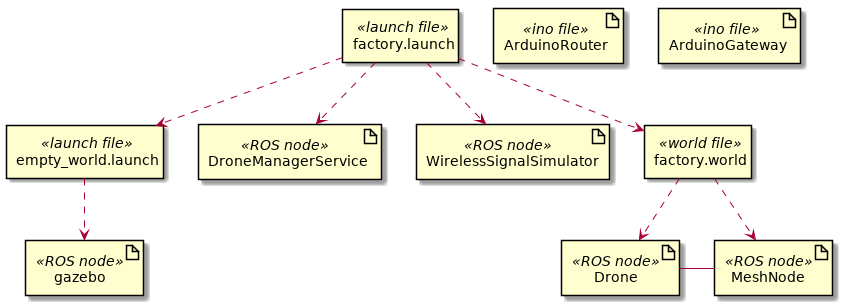
\includegraphics[width=\linewidth]{UML/out/DeploymentDiagram/DeploymentDiagram/DeploymentDiagram.png}\end{center}
	\caption{deployment diagram drone meshnetwerk}
	\label{fig:deploymentdiagram}
\end{figure}

\subsection{Ontwerpkeuzes met betrekking tot deployment}
\label{DetailedDesign:deployment:decisisions}

\subsubsection{Geen aangeboden mogelijkheid om drones los op te starten}
Er is voor gekozen om alleen via het factory.launch bestand de drones te kunnen starten. 
De factory.launch moet gebruikt worden omdat deze factory.world aanroept welke op zijn beurt de plugin start die de drones aanmaakt.  
In factory.world is het configureerbaar hoeveel gateway en router drones aangemaakt moeten worden.
Deze keuze is gemaakt omdat elke drone een uniek id moet hebben in de simulatie omdat elke motor zijn aansluiting publiceert aan de hand van dit id.

Om de gebruiker ervan te ontmoedigen is er daarom ook geen SDF bestand aanwezig waarmee normaal objecten in gazebo geladen worden. 

\section{Design Sub-Systeem Communicatie}
Het sub-systeem communicatie is verantwoordelijk voor de communicatie door het gebruik van mesh technologie.
Het subsysteem kan dit niet alleen en werkt daarom samen met andere subsystemen, welke zichtbaar zijn in het  \nameref{fig:componentdiagram}.
Het component communicatie bestaat ook weer uit kleinere componenten welke weergeven staan in het \nameref{fig:component:Communicatie}
  
\label{DetailedDesign:Communicatie}
\subsection{Component Diagram}
\label{DetailedDesign:CommunicatieComponentDiagram}
In de onderstaande afbeelding \ref{fig:component:Communicatie} staat het component diagram van de communicatie weergeven.
Het is een extractie uit het \nameref{fig:componentdiagram} 
\begin{figure}[H]
	\begin{center}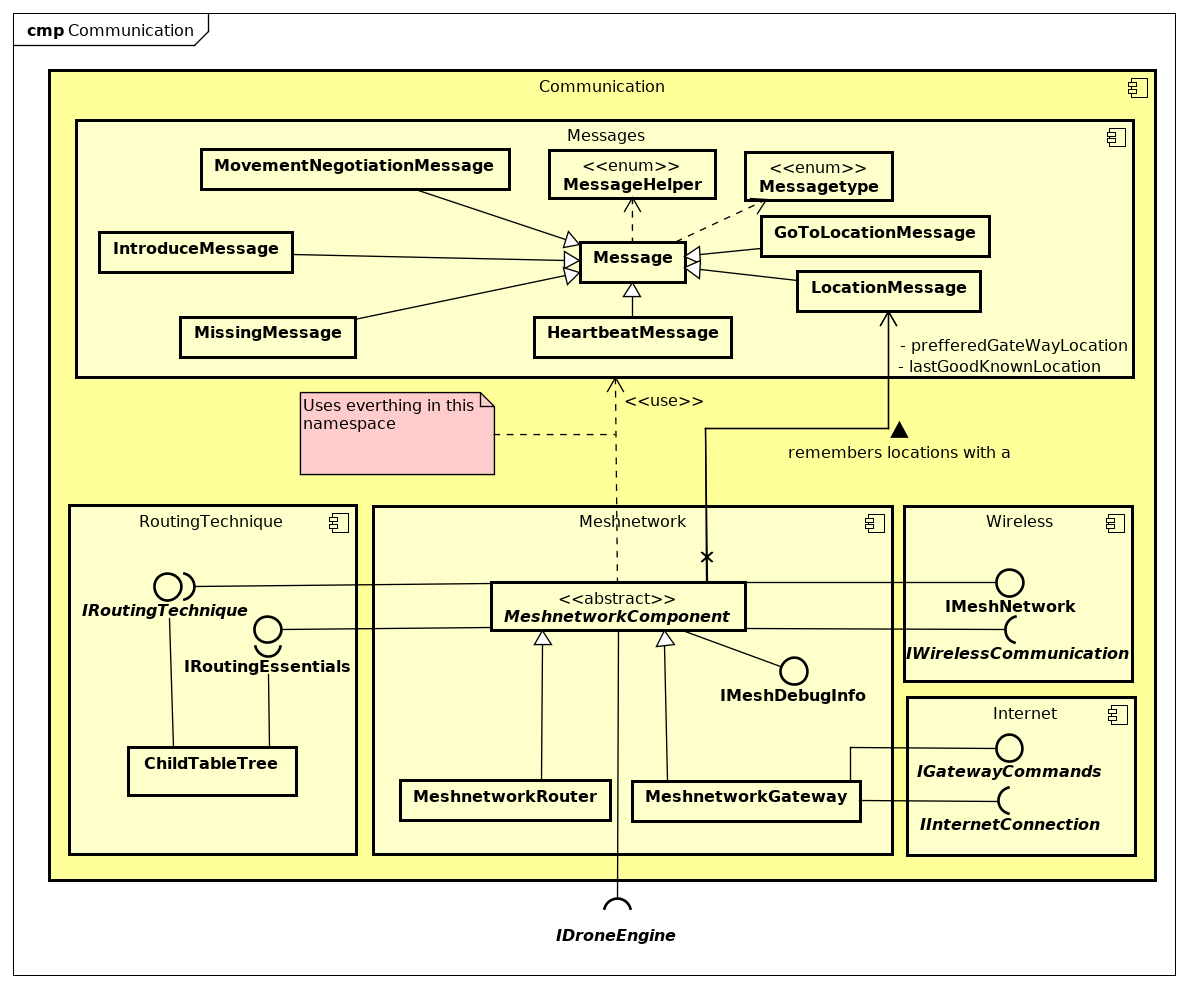
\includegraphics[width=\linewidth]{Afbeeldingen/CommunicationComponentDiagram.png}\end{center}
	\caption{Component diagram communicatie}
	\label{fig:component:Communicatie}
\end{figure}


\subsubsection{Meshnetwork}
\label{architectural:subcomponenten:Meshnetwork}
Dit component bevat de basis componenten voor het opbouwen van een meshnetwerk.

\subsubsection{MeshnetworkComponent}

\label{architectural:subcomponenten:MeshnetworkComponent}
Een MeshnetworkComponent is de basis van elk component in het meshnetwerk.
Het vereist routeringstechniek via de \nameref{architectural:interfaces:IRoutingTechnique}, een aansluiting naar een drone via \nameref{architectural:interfaces:IDroneEngine} en een vorm van draadloze communicatie via \nameref{architectural:interfaces:IWirelessCommunication}.
Hij maakt gebruikt van het component \nameref{architectural:subcomponenten:Messages} om te communiceren met andere MeshnetworkComponenten.

\subsubsection{MeshnetworkRouter}
\label{architectural:subcomponenten:MeshnetworkRouter}
Een meshnetwork router is een \nameref{architectural:subcomponenten:MeshnetworkComponent} die in staat is verbinding met andere nodes op te bouwen.
Zijn doel is om altijd verbinding te hebben met een \nameref{architectural:subcomponenten:MeshnetworkGateway}.
Als hij dit te lang niet heeft kan hij zich verplaatsen door aanspraak te maken op de DroneEngine.
Wanneer hij zich in een groep van andere Routers bevind zal hij eerst onderling onderhandelen wie er zich moet verplaatsen.

\subsubsection{MeshnetworkGateway}
\label{architectural:subcomponenten:MeshnetworkGateway}
De gateway is een \nameref{architectural:subcomponenten:MeshnetworkComponent} die in staat is een verbinding op te bouwen naar een punt buiten het meshnetwerk. In de huidige situatie kan dit via een internetverbinding die loopt via de interface \nameref{architectural:interfaces:IInternetConnection}. 

\subsubsection{Internet}
\label{architectural:subcomponenten:Internet}
Dit component bevat een high level interface om verbinding te maken en te verbreken met het internet.
Daarnaast biedt het een interface aan om berichten te ontvangen.

\subsubsection{Messages}
\label{architectural:subcomponenten:Messages}
Dit component betreft een verzameling van bericht samenstellingen die gebruikt worden voor de communicatie van het meshnetwerk.

\subsubsection{Message}
\label{architectural:subcomponenten:Message}
Een Message is de basis van elke bericht en bevat tenminste de volgende informatie:  Maker, zender, berichttype, ontvanger, geadresseerde. 
\subsubsection{GoToLocationMessage}
\label{architectural:subcomponenten:GoToLocationMessage}
Dit bericht bevat een locatie waar een drone zich naartoe moet verplaatsen.

\subsubsection{HeartbeatMessage}
\label{architectural:subcomponenten:HeartbeatMessage}
Dit bericht wordt gebruikt om de verbinding met anderen te onderhouden. Dit bericht maakt een hop per keer dat deze doorgestuurd wordt.

\subsubsection{IntroduceMessage}
\label{architectural:subcomponenten:IntroduceMessage}
Een introductie bericht wordt gebruikt door een node om schik voor te stellen aan alle andere nodes die dichtbij zijn. 

\subsubsection{LocationMessage}
\label{architectural:subcomponenten:LocationMessage}
Dit bericht wordt gebruikt om de huidige locatie van een node door te sturen naar een ander.

\subsubsection{MissingMessage}
\label{architectural:subcomponenten:MissingMessage}
Zodra een \nameref{architectural:subcomponenten:MeshnetworkComponent} de verbinding verliest met een ander gebruikt hij dit bericht om andere daarover te informeren.

\subsubsection{MovementNegotiationMessage}	
\label{architectural:subcomponenten:MovementNegotiationMessage}
Om onderling te onderhandelen tussen de nodes wie er actie moet ondernemen wordt dit bericht gebruikt.

\subsubsection{RoutingTechnique}
\label{architectural:subcomponenten:RoutingTechnique}
Dit component voorziet het meshnetwerk van een routing techniek wat dus inhoudt dat dit het component is die de communicatieroutes opbouwt naar andere punten in het netwerk.

\subsubsection{ChildTableTree}
\label{architectural:subcomponenten:ChildTableTree}
Deze techniek is een hybride meshnetwerk routing techniek waarbij een node de buren die deze heeft ziet als een kind.
Als een node een nieuw kind heeft vertelt hij dit aan zijn buren.
Omdat een node door zijn buren ook gezien wordt als kind registreren deze zijn nieuwe kind dus als kleinkind.
Hierdoor hoeft een node alleen maar te zoeken aan wie welk kind hij een bericht hoeft door te geven. 
De complexiteit van de routingtechniek neemt per stap in het netwerk af bij nodes met meerdere kinderen.
Als een drone zich verplaatst heeft wist deze het de opgebouwde geheugen van kinderen en kleinkinderen. 

\subsubsection{Wireless}
\label{architectural:subcomponenten:Wireless}
Dit component voorziet een \nameref{architectural:subcomponenten:MeshnetworkComponent} van een high level interface voor draadloze communicatie.
Als er een draadloos component wordt aangesloten moet deze hierop aangesloten worden. 
\subsection{Interfaces}
\label{DetailedDesign:CommunicatieComponentDiagram:interface}
Het communicatie component biedt zowel intern als extern interfaces aan. Deze worden hieronder omschreven.

\subsubsection{Extern aangeboden interface beschrijvingen}
\label{DetailedDesign:CommunicatieComponentDiagram:interface:extern}
Het communicatie component heeft drie extern aangeboden interfaces. De interface IMeshNetwork wordt aangeboden om berichten voor het meshnetwerk te kunnen ontvangen vanaf een aangesloten draadloos communicatie component. De interface IGatewayCommands wordt gebruikt voor het ontvangen van aansturing vanuit een extern punt naar een gateway. Tenslotte biedt het MeshnetworkComponent nog een interface aan met debuginformatie genaamd IMeshDebuginfo. Omdat deze laatste interface alleen maar getters bevat is besloten deze niet uitgebreid te behandelen.

\paragraph{IMeshNetwork}
\label{DetailedDesign:CommunicatieComponentDiagram:interface:IMeshnetwork}
De volgende functies worden aangeboden door de interface IMeshNetwork. 

\begin{lstlisting}
void OnMsg( const uint8_t* message );

const uint8_t getNodeID( ) const;
\end{lstlisting}

\subparagraph{OnMsg}
Deze functie geeft een antenne toegang tot een meshcomponent om berichten door te geven. Het bericht wordt opgegeven met een adresverwijzing tot de array waar het bericht in staat

\textbf{\textit{preconditie:}} Het meshcomponent heeft een thread gestart voor bericht afhandeling.

\textbf{\textit{postconditie:}} Het opgegeven bericht is behandeld door het meshcomponent.

\subparagraph{getNodeID}
Deze functie geeft de antenne door welk node id het meshcomponent bezit.

\textbf{\textit{preconditie:}} Het meshcomponent heeft een node id

\textbf{\textit{postconditie:}} Het id van het mehscomponent is doorgegeven.

\paragraph{IGatewayCommands }
\label{DetailedDesign:CommunicatieComponentDiagram:interface:IGatewayCommands}
De volgende functie wordt aangeboden door de interface IGatewayCommands. 

\begin{lstlisting}
void GoalRequestToDrone( const uint8_t ID, const float latitude,
			 const float longitude, const uint16_t height );
\end{lstlisting}

\subparagraph{SendGoalRequestToDrone}
Deze functie laat de aangesloten gateway een verzoek doen tot het verplaatsen van een drone. Er is nog geen ingebouwde functionaliteit om terug te geven of dit verzoek ook is aangekomen bij de drone. 

\textbf{\textit{preconditie:}} De gateway die het verzoek ontvangt heeft een route tot de drone die het verzoek moet ontvangen. 

\textbf{\textit{postconditie:}} De drone heeft het verzoek ontvangen en zal zich daar naartoe gaan verplaatsen

\subsubsection{Intern aangeboden interface beschrijvingen}
\label{DetailedDesign:CommunicatieComponentDiagram:interface:intern}

Intern worden er twee interfaces aangeboden. Het MeshnetworkComponent biedt een interface IRoutingEssentials aan waar basale communicatie functies in zitten om routeringstechnieken mogelijk te maken.  Ook wordt er een interface IRoutinTechnique door het subcomponent RoutingTechnique aangeboden.

\paragraph{IRoutingEssentials}

De volgende functies worden aangeboden door de interface IRoutingEssentials. 

\begin{lstlisting}

void searchOtherNodesInRange( )	

bool sendHeartbeat(uint8_t other);

\end{lstlisting}
\subparagraph{searchOtherNodesInRange}
Deze functie wordt aangeroepen om het component te verzoeken om te kijken of er andere nodes binnen bereik zijn.


\textbf{\textit{preconditie:}} Meshcomponent is voorzien van een draadloos communicatiemiddel die gestart is. 

\textbf{\textit{postconditie:}} Meshcomponent heeft een inventarisatie gemaakt van alles nodes binnen bereik. 

\subparagraph{sendHeartbeat}
Door het aanroepen van deze functie wordt er een hearbeat verzonden van het component naar een node met het opgegeven ID in de parameter.

\textbf{\textit{preconditie:}} Geadresseerde is bekend bij de routing techniek.

\textbf{\textit{postconditie:}} Routing techniek geeft terug welk adres het vervolg adres is voor het bericht.

\paragraph{IRoutingTechnique}

De volgende functies worden aangeboden door de interface IRoutingTechnique. 

\begin{lstlisting}
uint8_t getDirectionToNode( const uint8_t node );

void startRouting( );

void maintainRouting( );

void NodeMovedLocation( );

uint8_t cantCommunicateWithNode(const uint8_t node);

uint8_t OtherCantCommunicateWithNode(const uint8_t other, const uint8_t node);

void canCommunicateWithNode(const uint8_t node);

void OtherCanCommunicateWithNode(const uint8_t other, const uint8_t node);

const uint16_t getTableSize( );

const uint16_t getAmountOfChildren( );

const std::set< uint8_t > getSetOfChildren( );

const bool empty( );
\end{lstlisting}
\subparagraph{getDirectionToNode}
Deze functie is de functie waar de aanvragende interface het meeste belang bij heeft.
Deze functie verwacht een id van de geadresseerde node als parameter.
De routing techniek zal vervolgens uitzoeken naar welke node een bericht doorgegeven moet worden om het bericht aan te laten komen bij de geadresseerde.
Dit adres wordt terug gegeven als een return waarde. 

\textbf{\textit{preconditie:}} Geadresseerde is bekend bij de routing techniek.

\textbf{\textit{postconditie:}} Routing techniek geeft terug welk adres het vervolg adres is voor het bericht.

\subparagraph{startRouting}
De functie start routing wordt aangeroepen zodra de routing techniek moet beginnen met het opbouwen van communicatie routes.

\textbf{\textit{preconditie:}} Het communicatie waarover de routering gebeurd is beschikbaar

\textbf{\textit{postconditie:}} De node zich aangemeld bij andere nodes en kan adressen opslaan.

\subparagraph{maintainRouting}
Deze functie wordt herhaaldelijk aangeroepen in de software.
Het roept de routing techniek aan om een onderhoud te plegen aan de opgebouwde routing informatie.
Zo zal vaak het geval zijn dat de routing techniek controleert of de aansluitende nodes nog bestaan.

\textbf{\textit{preconditie:}} De routing techniek is gestart met routeren en heeft een lijst van beschikbare nodes.

\textbf{\textit{postconditie:}} Er is onderhoud uitgevoerd aan de lijst van beschikbare nodes.

\subparagraph{NodeMovedLocation} 
Deze functie wordt aangeroepen zodra de drone zich verplaatst heeft. Het is aan routing techniek om hier adequaat op te reageren.
In de huidige implementatie worden alle routes als ongeldig gezien waardoor de tabel geleegd wordt. 

\textbf{\textit{preconditie:}} Er is geen preconditie.

\textbf{\textit{postconditie:}} De routeringstechniek heeft de tabel bij adequaat bijgewerkt.


\subparagraph{cantCommunicateWithNode} 
Deze functie wordt aangeroepen als er geen connectie gelegd kan worden met een node. Deze functie geeft terug op hoeveel routes de node had in het netwerk. 

\textbf{\textit{preconditie:}} De node is aanwezig in de route tabel.

\textbf{\textit{postconditie:}} De route wordt verwijderd of als niet beschikbaar beschouwd.


\subparagraph{OtherCantCommunicateWithNode}
Deze functie wordt aangeroepen als een andere node aangeeft dat hij geen connectie kan maken met een node. Deze functie geeft terug op hoeveel routes de niet bereikbare node voorkomt. 

\textbf{\textit{preconditie:}} De node is aanwezig in de route tabel.

\textbf{\textit{postconditie:}} De route wordt verwijderd of als niet beschikbaar beschouwd.

\subparagraph{canCommunicateWithNode}
Zodra een node bevestiging heeft dat deze verbinding kan maken wordt deze functie aangeroepen. Als parameter wordt het adres meegegeven.

\textbf{\textit{preconditie:}} Er is bevestiging dat een node een directe verbinding heeft met een andere node.

\textbf{\textit{postconditie:}} De verbonden node wordt toegevoegd als direct route punt.
 
\subparagraph{OtherCanCommunicateWithNode}
De functie wordt aangeroepen als een andere node doorstuurt dat hij bevestiging heeft dat hij verbinding heeft met een nieuwe node in het netwerk. Als parameter wordt het adres meegegeven van zowel de node die aangeeft dat hij een verbinding heeft gevonden als het adres die hij gevonden heeft.

\textbf{\textit{preconditie:}}  Er is bevestiging dat een node een verbinding heeft met een andere node.

\textbf{\textit{postconditie:}}  De gevonden node wordt toegevoegd als route punt in het netwerk.


\subparagraph{getTableSize}
Deze functie geeft terug hoeveel routes er zich bevinden in de opgebouwde routing tabel.

\textbf{\textit{preconditie:}} Geen pre conditie.

\textbf{\textit{postconditie:}} Alle routes zijn geteld en de functie geeft dit aantal terug

\subparagraph{getAmountOfChildren}
In deze functie wordt het aantal gevonden direct aansluitende nodes geteld en terug gegeven.  

\textbf{\textit{preconditie:}}  Geen preconditie

\textbf{\textit{postconditie:}} Het aantal direct aansluitende nodes is geteld en en dit aantal is terug gegeven.

\subparagraph{getSetOfChildren}
Hier wordt een set gemaakt met id's van direct aansluitende nodes 
\textbf{\textit{preconditie:}} Geen preconditie

\textbf{\textit{postconditie:}} Er is een set met de id's van alle nodes waar een directe verbinding mee gevonden is

\subparagraph{empty}
Deze functie geeft een boolean terug welke aangeeft of de tabel leeg is.
Dit is een aparte functie omdat het scheelt in complexiteit ten opzichte van het tellen van een tabel en die vergelijken met 0.
  
\textbf{\textit{preconditie:}} Geen preconditie

\textbf{\textit{postconditie:}} Er is een check gedaan of de lijst leeg is en dit wordt terug gegeven.

\subsection{Sequence Diagrams}
\label{DetailedDesign:Communicatie:sequence}
Hier worden aan de hand van sequence diagrammen communicatie wegen omschreven die gebruikt worden tussen verschillende nodes in het netwerk.

\subsubsection{Heartbeat van router naar gateway met directe verbinding}
\label{DetailedDesign:Communicatie:sequence:heartbeatrouter->gateway}
Om duidelijk te maken hoe een bericht van een node naar een gateway komt wordt het scenario van een heartbeat uitgewerkt in een direct verbinden.
Deze weg van communicatie wordt voor alle directe berichten het zelfde uitgevoerd.
Dat maakt het overbodig om voor elk type bericht een sequence diagram uit te werken
\begin{figure}[H]
	\begin{center}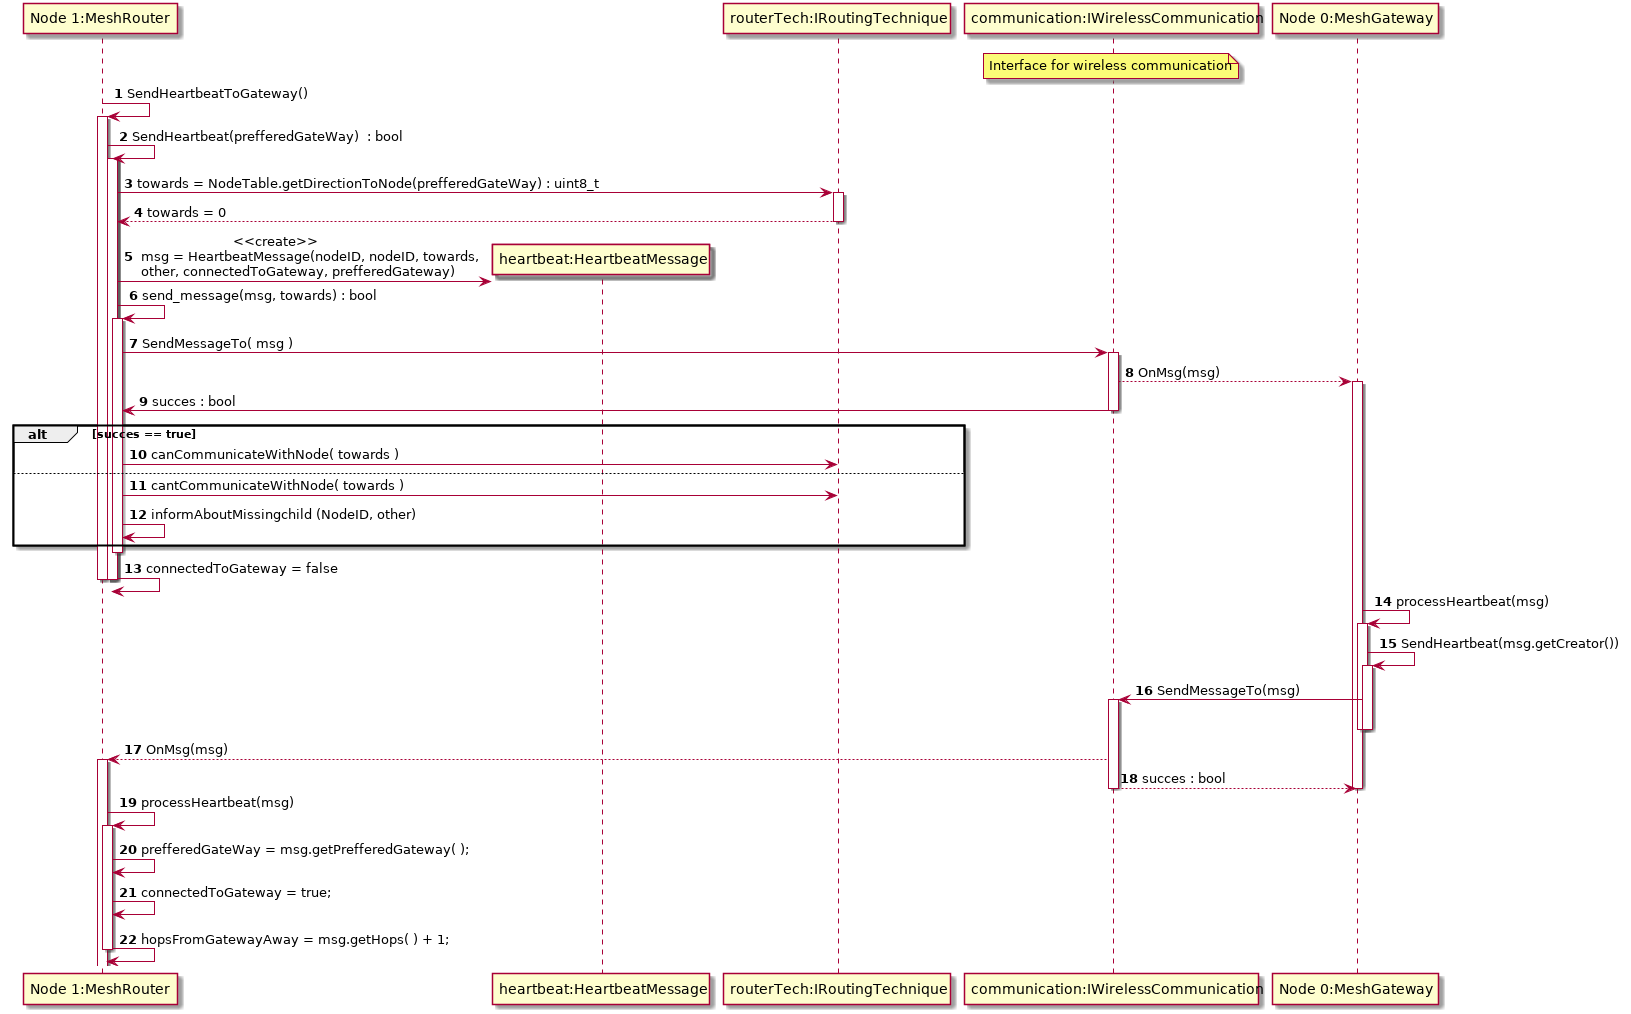
\includegraphics[width=.97\linewidth]{UML/out/Communication/Sequence/RouterDirectNaarGatewayHeartbeat/RouterDirectNaarGatewayHeartbeat.png}\end{center}
	\caption{Sequence diagram van een heartbeat bericht van een router naar een gateway met een directe onderlinge verbinding.}
	\label{fig:communication:sequence:sequence:heartbeatrouter->gateway}
\end{figure}
In diagram \ref{fig:communication:sequence:sequence:heartbeatrouter->gateway} is de flow zichtbaar van een router die een heartbeat bericht verstuurd naar een gateway en daar ook weer response op krijgt.
Op het moment dat een router het bericht om een heartbeat te versturen naar de gateway zal hij dit altijd doen naar de gateway waar hij een voorkeursverbinding (prefferedGateway) mee heeft.
Hij zal aan de aangesloten routeringstechniek vragen of er een route mogelijk is naar de router een aan wie hij zijn bericht dan moet afgegeven.
In het geval van deze sequence diagram heeft de router een directe verbinding met de gateway en is in stap 4 te zien dat het teruggegeven adres 0 is het adres van de gateway.

Vervolgens maakt de router een heartbeat bericht aan die het via de \nameref{architectural:interfaces:IWirelessCommunication} interface verstuurd naar de Gateway.
De router geeft door aan de routeringstechniek in stap 10 of 11 of het zenden wel of niet gelukt is op basis van de succes feedback uit stap 9.
Als het niet lukt geeft hij dit ook door aan zijn aangesloten punten in stap 12. 
De werking hiervan is terug te vinden in \nameref{DetailedDesign:Communicatie:sequence:contactverlies}
Als laatste voordat de router zijn functie verlaat zet hij in stap 13 de boolean die bijhoudt of verbinding is met de gateway (connectedToGateway) op false omdat hij verwacht dat er reactie komt van de gateway die het weer op true zet.

Bij stap 8 is het gelukt om het bericht te versturen naar de gateway die daar via zijn eigen \nameref{architectural:interfaces:IWirelessCommunication} interface het bericht ontvangt.
Er is voor gekozen om deze interface maar één keer weer te geven in de tabel om het overzichtelijk te houden.
De reactie van een gateway op een heartbeat is altijd dat er een heartbeat wordt teruggestuurd naar de zender. 
De functie SendHeartbeat(uint8\textunderscore t) in stap 15 werkt gelijk aan die van stap 2 en is daarom niet opnieuw uitgewerkt.

Stap 17 is het moment dat de router weer response heeft van de gateway.
Hij stelt op basis van de inhoud van het bericht het ID van de gateway in als prefferedGateway, zet de boolean connectedToGateway weer op true en registreert hoeveel hops het bericht nodig had om aan te komen.

\subsubsection{Heartbeat van gateway naar een router via een andere router}
\label{DetailedDesign:Communicatie:sequence:heartbeatgateway->router->router}

\begin{figure}[H]
	\begin{center}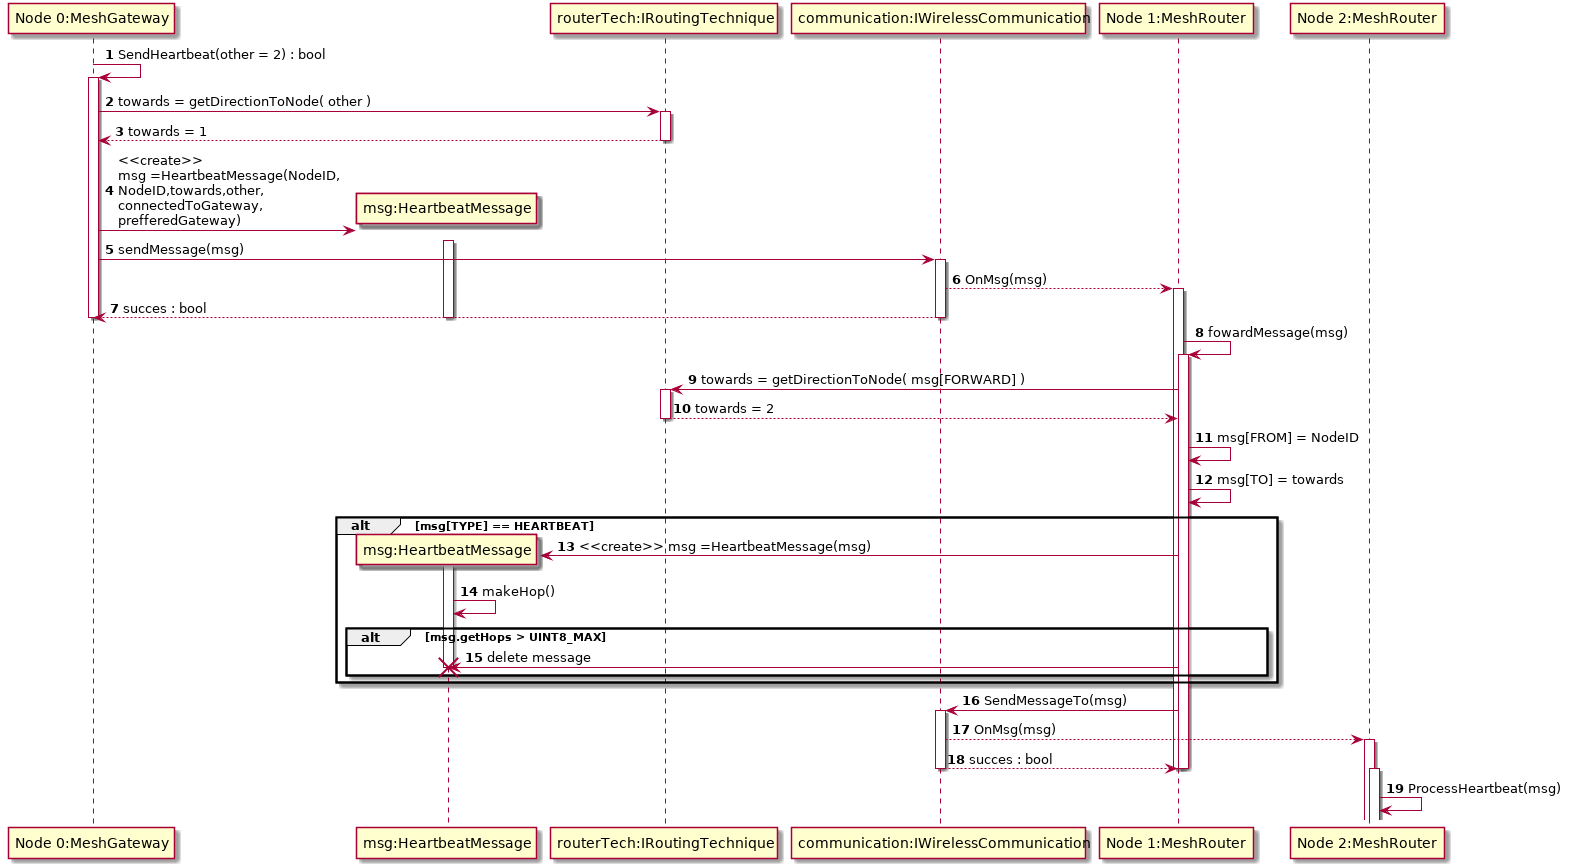
\includegraphics[width=\linewidth]{UML/out/Communication/Sequence/ForwardHeartbeat/ForwardHeartbeat.png}\end{center}
	\caption{Sequence diagram van een heartbeat bericht van een gateway naar een router via een andere router.}
	\label{fig:communication:sequence:sequence:heartbeatgateway->router->router}
\end{figure}
Diagram \ref{fig:communication:sequence:sequence:heartbeatgateway->router->router} laat zien hoe een heartbeat verstuurd wordt vanaf een gateway naar een router via een andere router.
Er is gekozen om de flow van een heartbeat bericht te laten zien omdat deze bij een forward ook een hop extra krijgt en daarmee het meest complex is.
Elke node heeft een eigen instantie van een routeringstechniek en draadloze communicatie, in deze diagram is gekozen om dezelfde te gebruiken om de leesbaarheid goed te houden.

Bij stap 3 is zichtbaar dat de routeringstechniek bij aanvraag voor een route naar node 2 een adres teruggegeven wordt van node 1 omdat via deze weg het bericht doorgegeven moet worden.
Vanaf stap 8 is zichtbaar wat er gebeurd als een bericht doorgestuurd moet worden.
Bij stap 9 wordt er eerst gekeken of er een route is naar de geadresseerde en aan wie het bericht dan doorgegeven moet worden.
Node 1 heeft een directe verbinding met node 2 dit wordt dan ook als adres doorgegeven in stap 10.
Vervolgens past de meshrouter het bericht aan dat zodat de zender en ontvanger weer juist staan. 
De waardes waar in staat wie de geadresseerde en maker van het bericht zijn blijven onaangepast.
Als het bericht van het type heartbeat is wordt deze apart genomen om er in stap 14 een hop bij op te tellen.
Als een heartbeat bericht meer hops heeft gemaakt dan dat er in de waarde van hop past wordt het bericht verwijderd en de flow gestopt.

In stap 16 wordt het bericht doorgestuurd naar de geadresseerde.
Als het bericht een heartbeat was wordt deze doorgestuurd anders wordt het aangepaste bericht verstuurt.

\subsubsection{Heartbeat van een router naar een andere router}
\label{DetailedDesign:Communicatie:sequence:heartbeatrouter->router}
\begin{figure}[H]
	\begin{center}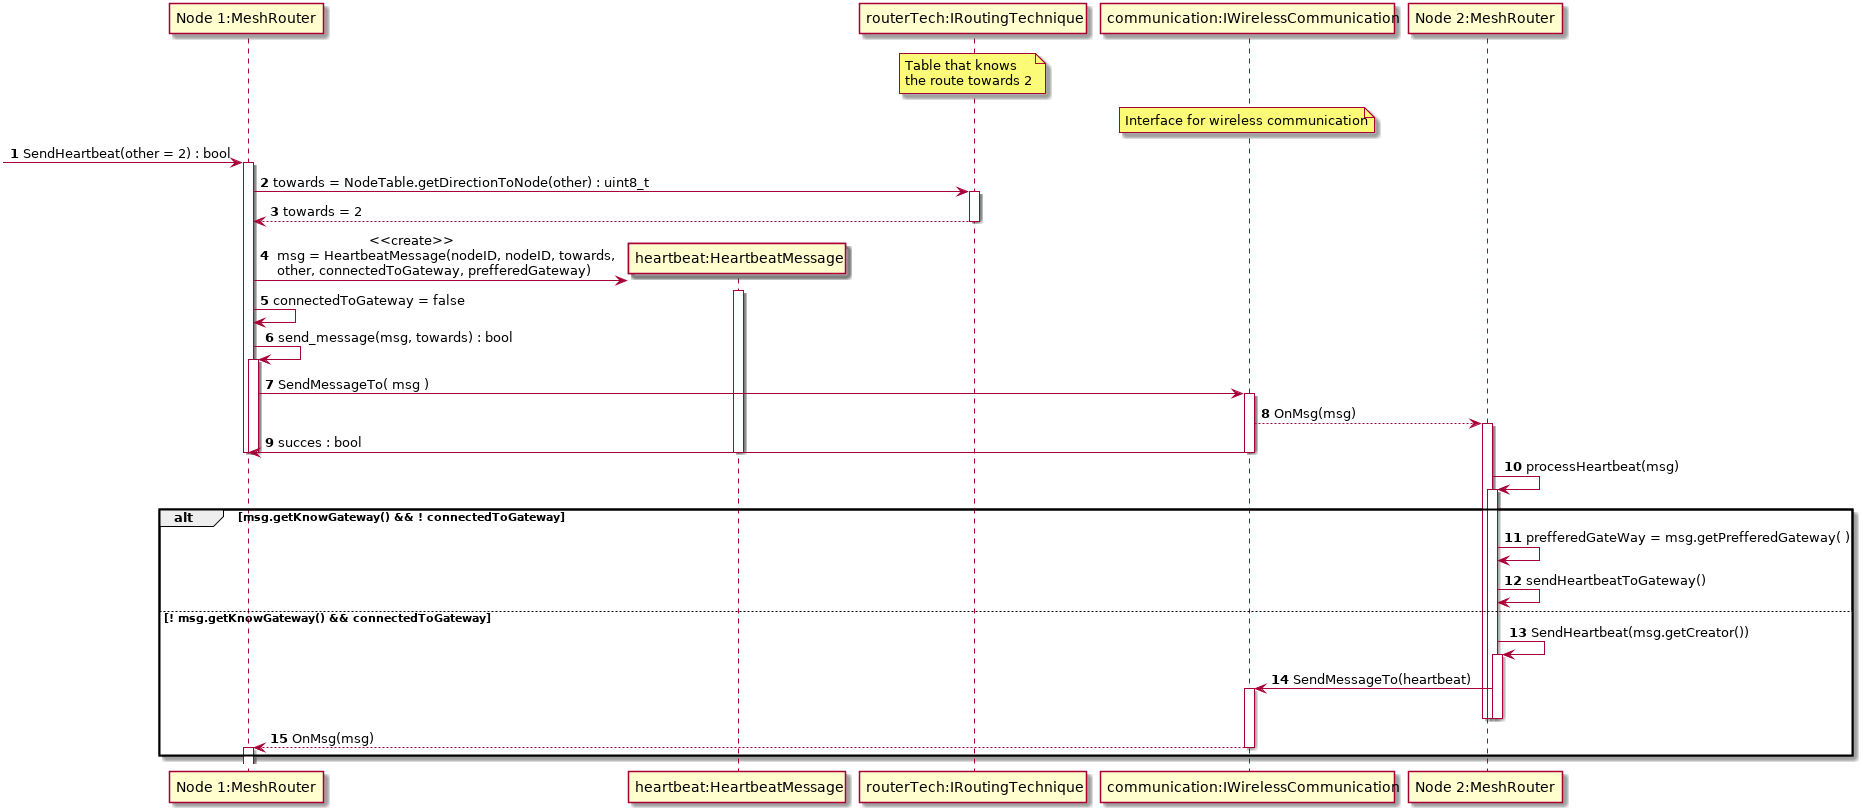
\includegraphics[width=\linewidth]{UML/out/Communication/Sequence/RouterHeartbeatRouter/RouterHeartbeatRouter.png}\end{center}
	\caption{Sequence diagram van een router die een heartbeat stuurt naar een router.}
	\label{fig:communication:sequence:sequence:router->router}
\end{figure}
In de bovenstaande sequence diagram \ref{fig:communication:sequence:sequence:router->router} wordt de flow behandeld van een heartbeat van een router naar een andere router.
De keuze om dit in een sequence diagram uit te werken is om te laten zien dat er niet in elke scenario een reactie bericht verwacht hoeft te worden.

In stap 11 en 12 is bijvoorbeeld de afhandeling te zien als de zendende router verbinding heeft met een gateway en de ontvangende router niet.
In dit scenario gaat de router geen bericht terugsturen maar stelt hij de gateway die de zendende router heeft in als voorkeur en probeert een heartbeat te versturen naar deze gateway.    
Als het scenario omgedraaid is en de zendende router heeft geen verbinding met een gateway maar de ontvangende router wel stuurt hij juist wel een heartbeat terug. 
De zendende router zal hierdoor de zelfde stappen gaan uitvoeren als stap 11 en 12 waardoor hij weer een verbinding opbouwt met een gateway.

Dit houdt dus ook in dat als beide routers geen verbinding hebben met een gateway, of allebei wel, dat ze geen response sturen op een heartbeat.

\subsubsection{Informatieverspreiding bij verliezen contact met andere node}
\label{DetailedDesign:Communicatie:sequence:contactverlies}
Op het moment dat een node doorheeft dat er een verbinding verloren is met een andere node gaat hij de op hem aangesloten nodes daarover informeren. Dit zodat ieder andere node zijn routingstabel kan updaten 
\begin{figure}[H]
	\begin{center}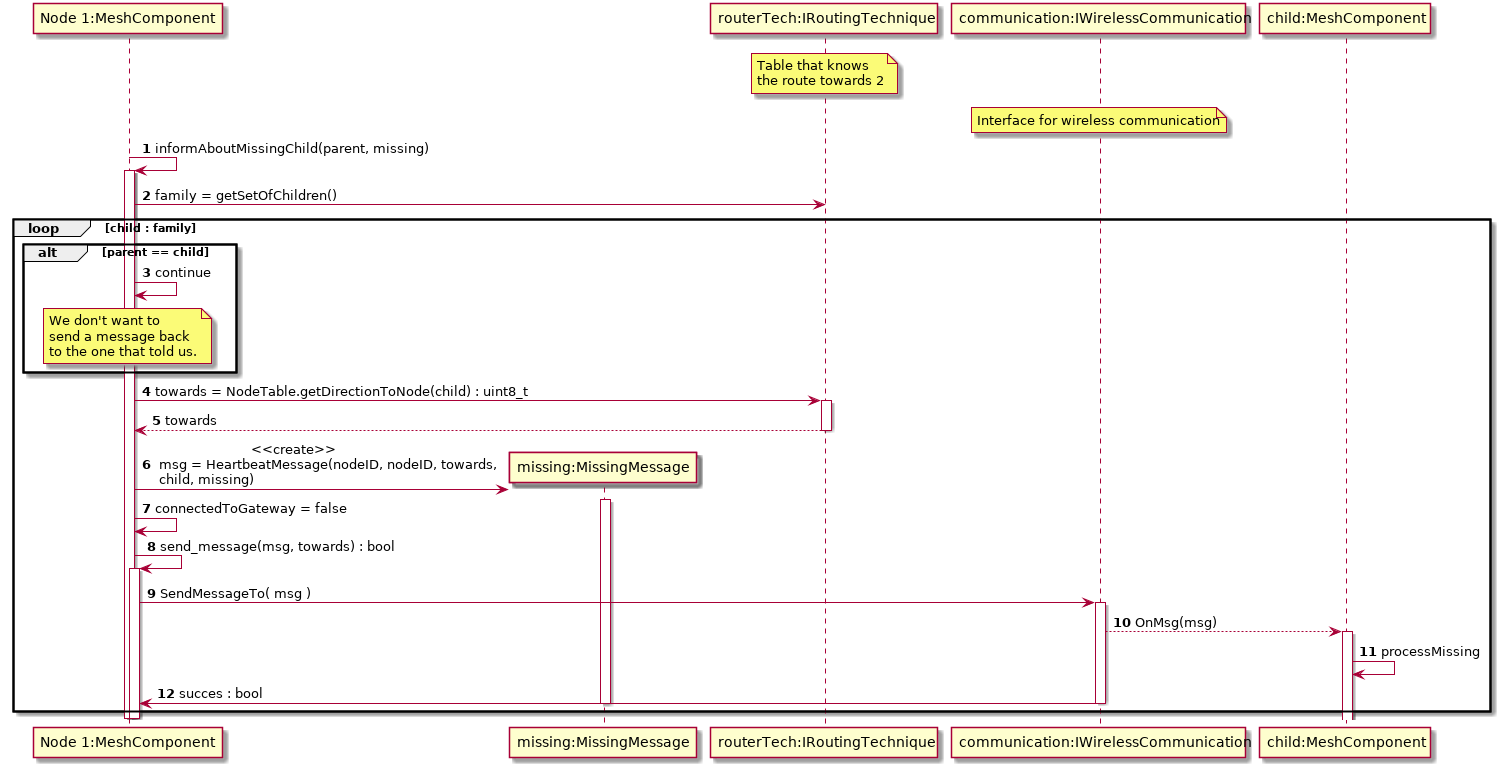
\includegraphics[width=\linewidth]{UML/out/Communication/Sequence/LostConnectionWithOther/LostConnectionWithOther.png}\end{center}
	\caption{Sequence diagram van een component die zijn aangesloten nodes op de hoogte brengt van een verloren node.}
	\label{fig:communication:sequence:contactverlies}
\end{figure}

De eerste stap die een meshcomponent onderneemt is het raadplegen van de routeringstechniek of er direct aangesloten nodes zijn.
Per aangesloten node verstuurt het component een bericht dat er een node geen verbinding meer wil maken.
Een uitzondering is als de direct aangesloten node degene is die het component geïnformeerd heeft over het feit van de vermissing.
Die ontvangt geen bericht aangezien deze natuurlijk al op de hoogte is.


\subsection{Activity Diagrammen}
\label{DetailedDesign:Communicatie:Activity}

Aan de hand van de onderstaande activity diagrammen wordt de flow van de communicatie applicatie uitgelegd. 
In het component zijn twee soorten applicaties beschikbaar een router en een gateway. 
Deze worden eerst apart behandeld daarna zal de rest van het component aan bod komen.

Voor elk activity diagram telt dat er onder het diagram een begeleidende tekst is toegevoegd.

\subsubsection{Activity diagrammen router}
\label{DetailedDesign:Communicatie:Activity:router}

Eerst wordt de algemene flow van de router applicatie toegelicht vervolgens zullen protocollen worden toegelicht die optreden in bepaalde situaties.

\paragraph{Meshnetwerk router applicatie}
\label{DetailedDesign:Communicatie:Activity:router:applicatie}
De onderstaande flow zichtbaar in \autoref{fig:communication:activity:meshrouter} laat de algemene flow zien van de router applicatie. 


\begin{figure}[H]
	\begin{center}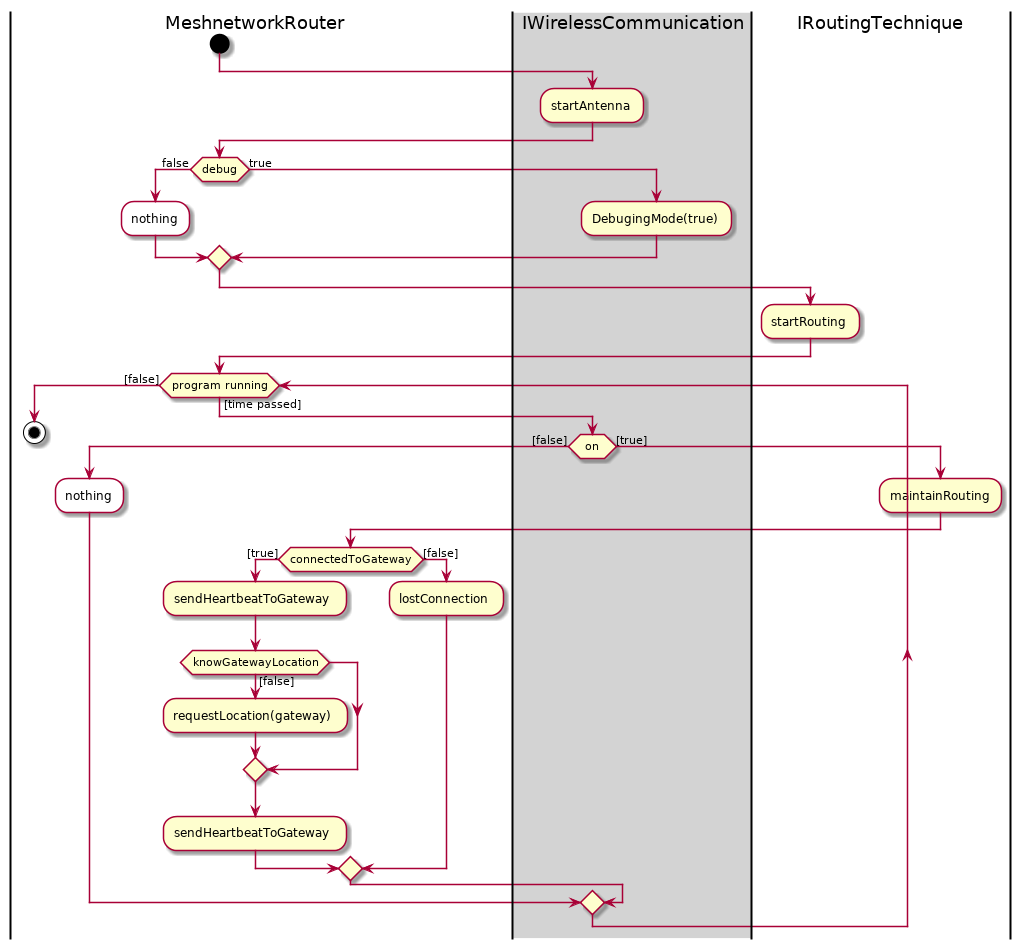
\includegraphics[width=.83\linewidth]{UML/out/Communication/activity/MeshRouter/MeshRouter.png}\end{center}
	\caption{Activity diagram meshnetwerk router applicatie.}
	\label{fig:communication:activity:meshrouter}
\end{figure}


Zodra het programma start wordt als eerste de antenne aan gezet en wanneer dit geactiveerd is ook de de debug stand van de antenne. 
Nadat deze is opgestart wordt kenbaar gemaakt aan de routeringstechniek dat deze ook kan starten met het opbouwen van routes.

Nu deze twee zijn opgestart kan de basis lus van het programma beginnen. 
Zolang het programma draait wordt deze lus herhaald.

Elke  keer zodra het programma op dit punt aankomt wacht het 10(instelbaar) seconden.
Hierna controleert de router of de aangesloten antenne nog aan staat. 
Als dit niet zo is begint de lus opnieuw.
Als de antenne wel aan staat wordt er een verzoek gedaan aan de routeringstechniek om onderhoudt te plegen.

Vervolgens zijn er twee paden mogelijke op basis van het feit of er verbinding is met een gateway.
Als er geen verbinding is wordt het protocol opgestart voor een verloren verbinding.
Hoe dit protocol werkt wordt apart toegelicht in het hierop volgende diagram.

Wanneer er wel verbinding is met een gateway wordt er gekeken  of de router ook op de hoogte is van de locatie van de router.
Als hij dit nog niet weet vraagt hij deze op bij de gateway.
Tenslotte wordt er een heartbeat verstuurt naar de gateway.

\pagebreak
\paragraph{Meshnetwerk router protocol bij verloren verbinding}
\label{DetailedDesign:Communicatie:Activity:verloren}
In het diagram getoond in \autoref{fig:communication:activity:verlorenverbinding} wordt het protocol uitgelegd die een router uitvoert zodra deze zijn verbinding heeft verloren met een gateway.

\begin{figure}[H]
	\begin{center}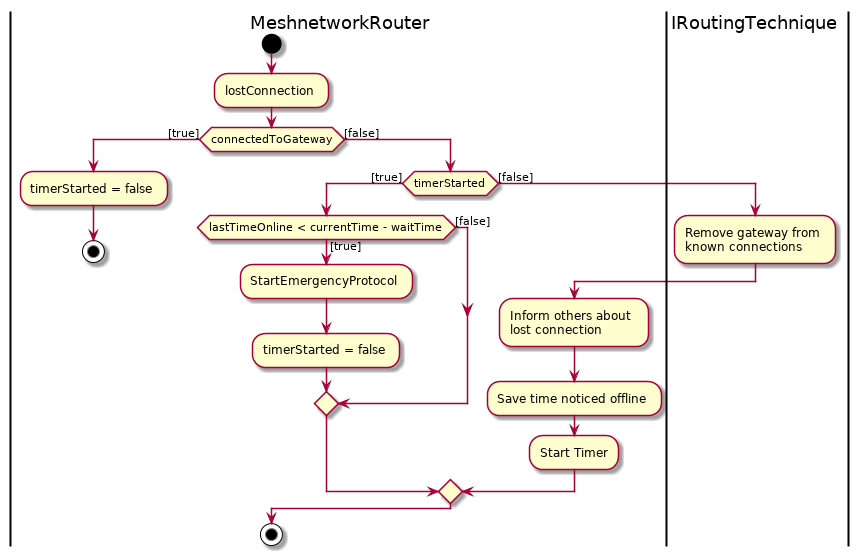
\includegraphics[width=1\linewidth]{UML/out/Communication/activity/LostConnection/LostConnection.png}\end{center}
	\caption{Activity diagram verloren verbinding protocol.}
	\label{fig:communication:activity:verlorenverbinding}
\end{figure}

Het protocol start op met het nogmaals checken of de gateway geen verbinding heeft.
Als er nog steeds geen verbinding is wordt er gekeken of er al een timer gestart is die bijhoudt hoelang er al geen verbinding meer is.

Als er nog geen timer gestart is wordt de routeringstechniek op de hoogte gebracht dat de verbinding verloren is met de gateway.
Vervolgens worden de direct aangesloten nodes ook op de hoogte gebracht van de verloren verbinding.
Tenslotte  wordt er een timer gestart door een boolean te schakelen en de huidige tijd op te slaan daarna wordt de functie verlaten.

Als er al wel een timer gestart is wordt er gekeken of de tijd die een node zonder verbinding mag zitten al verstreken is.
Als deze tijd nog niet verstreken is wordt de functie verlaten.

Wanneer de tijd wel verstreken is wordt het noodprotocol opgestart die in de volgende paragraaf beter wordt toegelicht.
Zodra dit protocol is uitgevoerd wordt de timer weer uitgezet zodat deze in een volgende lus weer opnieuw gaat lopen.
\pagebreak
\paragraph{Meshnetwerk router noodprotocol}
In \autoref{fig:communication:activity:nood} wordt het uitgevoerde protocol toegelicht die wordt uitgevoerd wanneer een node te lang zonder verbinding zit.

\begin{figure}[H]
	\begin{center}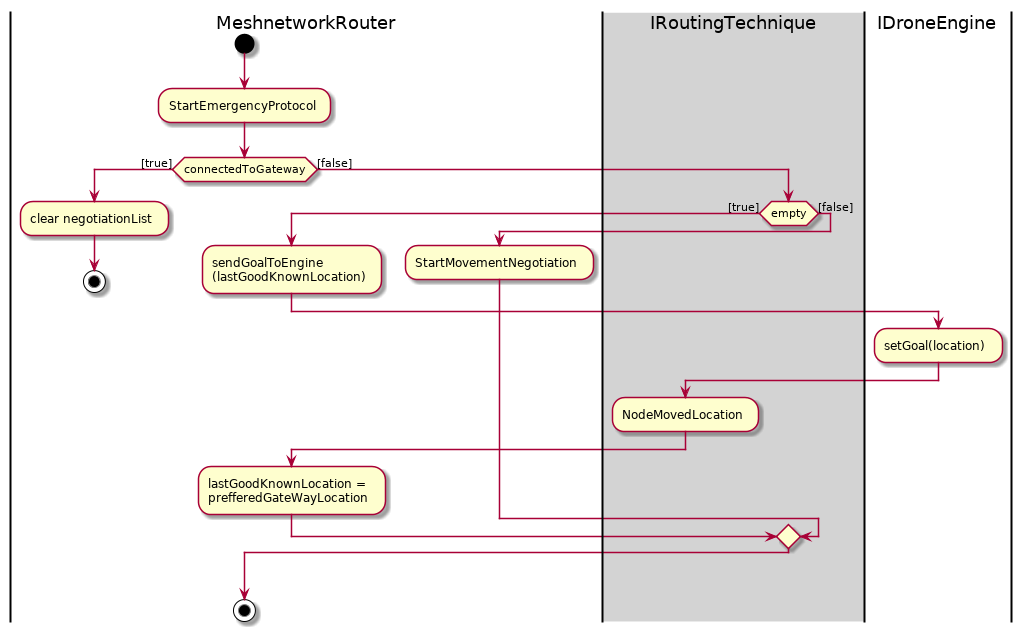
\includegraphics[width=\linewidth]{UML/out/Communication/activity/EmergencyProtocol/EmergencyProtocol.png}\end{center}
	\caption{Activity diagram noodprotocol.}
	\label{fig:communication:activity:nood}
\end{figure}

Het noodprotocol begint met een laatste check of de node ondertussen alweer verbinding heeft 
als dit zo is wordt het protocol niet uitgevoerd en de onderhandelingslijst leeg gehaald.

Wanneer er nog steeds geen verbinding is gelegd met een gateway wordt het protocol gestart.
Eerst wordt de routing techniek geraadpleegd of er nog andere nodes verbonden zijn met deze node.

Als dat niet zo is wordt er een verzoek gestuurd naar de drone om zich te gaan verplaatsen naar de locatie die als laatste gemarkeerde is als goede locatie.
Nadat deze verplaatst is wordt de locatie van de gateway ingesteld als laatst bekende goede locatie.
Ook wordt de routeringstechniek op de hoogte gesteld dat er een verplaatsing heeft plaats gevonden.
Als dit allemaal is uitgevoerd wordt dit protocol gesloten.

Wanneer er wel andere nodes verbonden zijn met deze node dan moeten deze onderling gaan onderhandelen wie er een verplaatsing moet gaan uitvoeren om zo efficiënt mogelijk het netwerk proberen te herstellen. Deze werking is apart uitgelegd in de hier opvolgende activity diagram \ref{fig:communication:activity:verplaatsingsonderhandeling}. Nadat deze onderhandelingen zijn afgelopen wordt het noodprotocol afgesloten zodat het netwerk even een moment heeft een poging te doen zichzelf te herstellen.
\pagebreak
\paragraph{Meshnetwerk router verplaatsingsonderhandeling}
\autoref{fig:communication:activity:verplaatsingsonderhandeling} laat de flow zien die een enkele node neemt wanneer deze start met onderhandelen over wie er een verplaatsing moet uitvoeren.


\begin{figure}[H]
	\begin{center}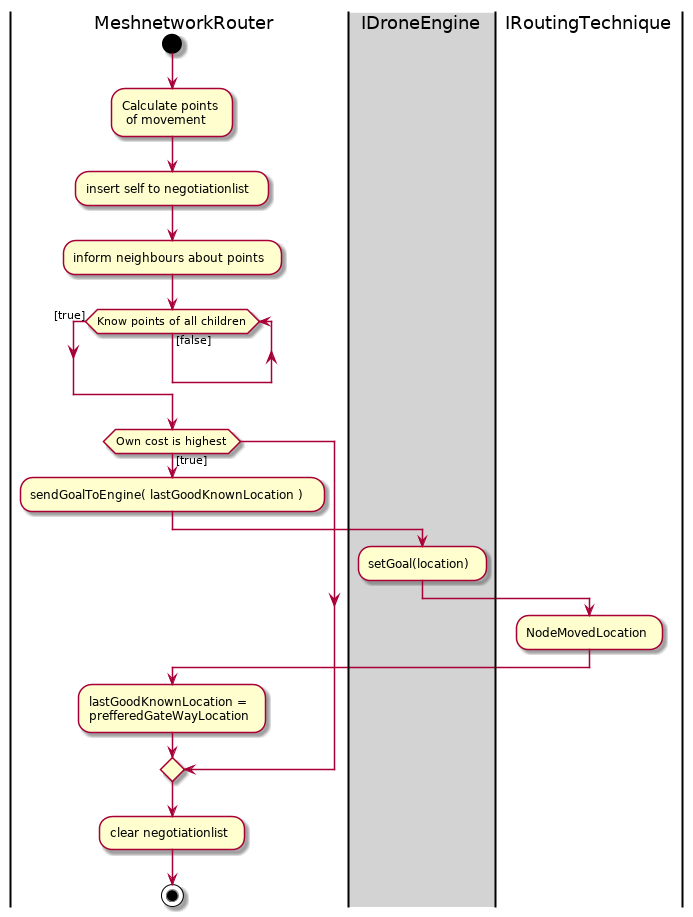
\includegraphics[width=.6\linewidth]{UML/out/Communication/activity/MovementNegotiation/MovementNegotiation.png}\end{center}
	\caption{Activity diagram verplaatsingsonderhandeling}
	\label{fig:communication:activity:verplaatsingsonderhandeling}
\end{figure}
De flow begint met het berekenen hoeveel punten de beweging van de node scoort.
In de opgeleverde applicatie worden de verplaatsingpunten op twee factoren gebaseerd.
Het aantal punten die een node krijgt staat gelijk aan de afstand die het heeft hemelsbreed met de gateway.

Hiervoor wordt Pythagoras gebruikt om de afstand te berekenen wat zichtbaar is in \autoref{math:pythgoras:locatie} 
\begin{equation}
\label{math:pythgoras:locatie}
afstand =   \sqrt{(x_{gateway} - x_{postitie})^2+(y_{gateway} - y_{postitie})^2+(z_{gateway} - z_{postitie})^2}							
\end{equation}

In deze vergelijking is de positie van een drone vertaald naar een cartesiaanse waarde daarom worden er x,y,z waardes gebruikt die slaan op de latitude, longitude en height waardes van de drone.

Een voorwaarde is wel dat de locatie waar de node zich naartoe wil gaan verplaatsen niet bezet wordt door een andere node. Als dit zo is worden de punten op -1 gezet waardoor die automatisch niet meer mee doet omdat er gekeken omdat het minimale aantal punten 0 is.

Hierna voegt de node zichzelf toe in de onderhandellijst en maakt hij zijn score bekend aan zijn aangesloten nodes.
Zodra de node dit bekend heeft gemaakt wacht hij tot de andere nodes dit ook hebben gedaan.

Als dit zover is kijkt de node of hij de hoogste score heeft in een lijst.

Wanneer een node de hoogste score heeft verzoekt hij de drone om zich te verplaatsen naar de laatst bekende goede locatie. Ook maakt de node dit bekend aan de routeringstechniek. 
Vervolgens stelt de node de locatie van de gateway in als laatste bekende goede locatie.

Tenslotte maakt de node altijd aan het einde van de onderhandeling de lijst waar alle onderhandel waardes in staan. 

\subsubsection{Activity diagrammen gateway}
\label{DetailedDesign:Communicatie:Activity:gateway}
In het volgende stuk worden de activity diagrammen behandeld die specifiek betrekking hebben op de gateway applicatie. Eerst wordt de algemene flow van de applicatie behandeld en daarna flows binnen de applicatie

\paragraph{Meshnetwerk gateway applicatie}
Deze paragraaf beschrijft de algemene flow van de gateway applicatie. 
\label{DetailedDesign:Communicatie:Activity:gateway:applicatie}
\begin{figure}[H]
	\begin{center}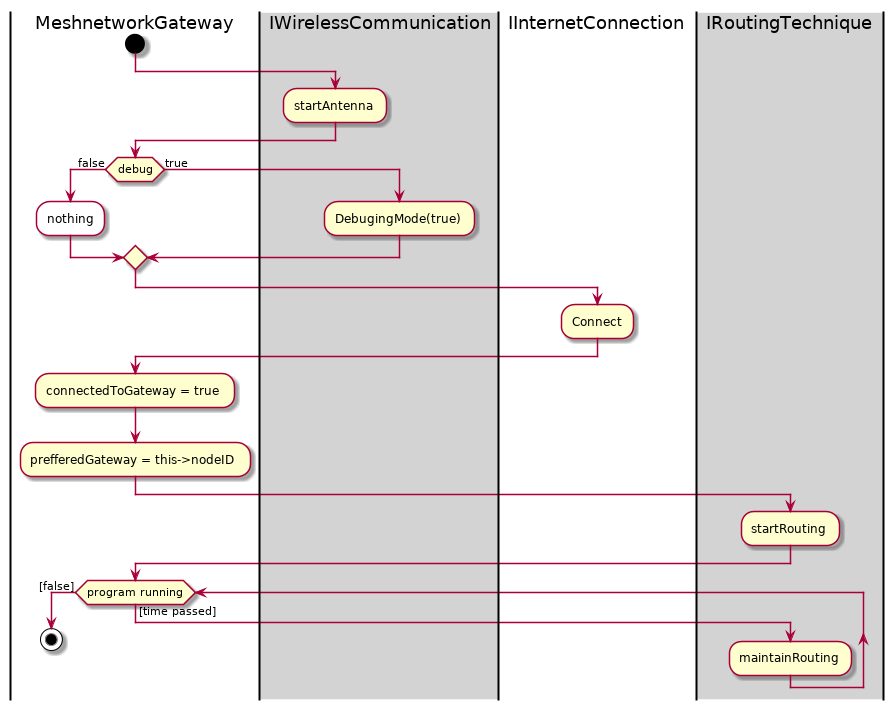
\includegraphics[width=.8\linewidth]{UML/out/Communication/activity/MeshGateway/MeshGateway.png}\end{center}
	\caption{Activity diagram meshnetwerk Gateway applicatie.}
	\label{fig:communication:activity:gateway}
\end{figure}

Zodra de gateway begint start hij meteen de antenne op van de draadloze communicatie.
Als debug aan staat verzoekt hij deze stand van de antenne om aan te gaan.
Na het starten van de antenne zoekt de gateway een verbinding op met het internet via de aangesloten \nameref{architectural:interfaces:IInternetConnection} om zo aansturen vanuit een extern punt van het meshnetwerk mogelijk te maken.

Daarna stelt hij de variabelen in die gebruikt worden in het netwerk om routers een weg naar de router toe te laten vinden. Voor nu worden de waarde dat er een verbinding is met de gateway altijd op waar gezet. In de toekomst kan dit nog veranderd worden op basis van het feit of er een internetverbinding is opgezet. 

Tenslotte begint de gateway met een verzoek naar de routeringstechniek om te starten met routeren. Waarna de gateway alleen nog periodiek een verzoek zal sturen om de routering te onderhouden.

\subsubsection{Meshnetwerk algemene applicatie}
Dit volgende stuk beschrijft de flows in de applicatie die zowel de router als de gateway volgen. 

\paragraph{Meshnetwerk flow bij ontvangst bericht}
\label{DetailedDesign:Communicatie:Activity:meshcomponent:onmsg}
Deze paragraaf beschrijft acties die de applicatie onderneemt bij het ontvangen van een bericht. 
\begin{figure}[H]
	\begin{center}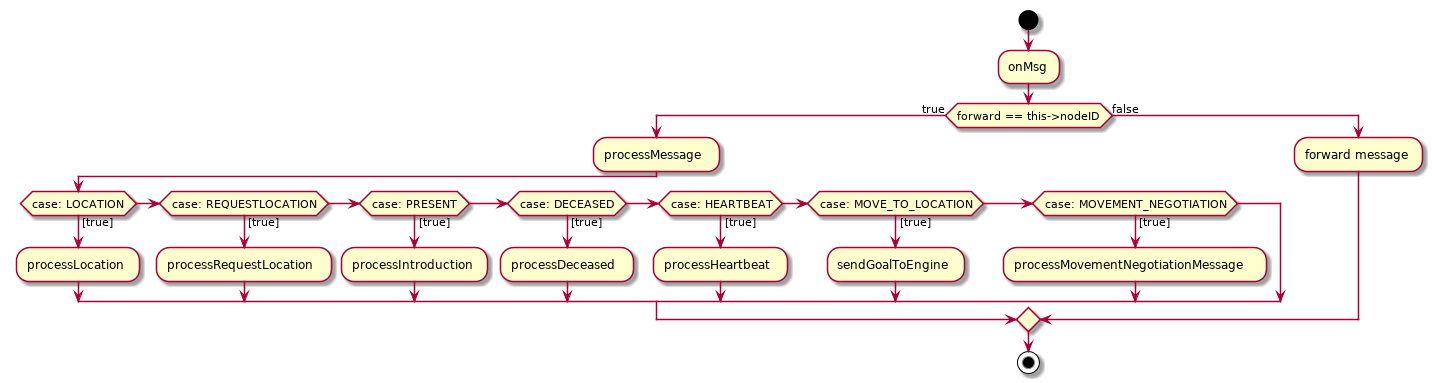
\includegraphics[width=.8\linewidth]{UML/out/Communication/activity/processMessage/processMessage.png}\end{center}
	\caption{Activity diagram meshnetwerk flow ontvangen bericht}
	\label{fig:communication:meshcomponent:onmsg}
\end{figure}

In het acitvity diagram is te zien dat er bij het ontvangen van een bericht eerst wordt gekeken of het bericht geadresseerd is voor de ontvangende node.
Als die niet zo is dan wordt het bericht doorgestuurd naar een volgend punt.

Wanneer het wel geadresseerd is voor de ontvangende node dan gaat het de functie in om het bericht te verwerken. Hoe het bericht verwerkt wordt is afhankelijk van het type die het bericht bij zich draagt. Dit wordt gedaan aan de hand van een switch case.

\paragraph{Routeringstechniek voor het vinden van een pad tot het adres}
\label{DetailedDesign:Communicatie:Activity:routeringtechniek:aanvraag}
In het communicatie component is een routeringstechniek aanwezig voor het vinden van een route tot een pad. Hoe deze techniek het volgende adres vindt in de route wordt getoond in het volgende activity diagram. 

\begin{figure}[H]
	\begin{center}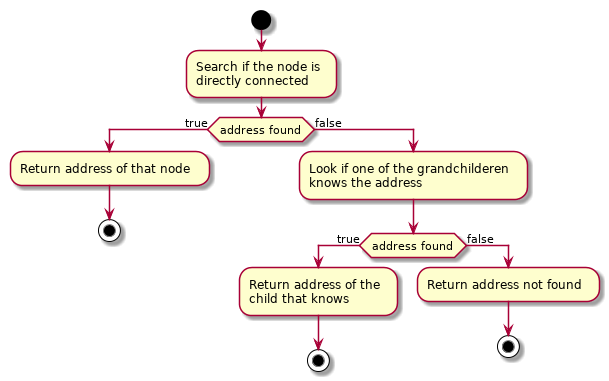
\includegraphics[width=.45\linewidth]{UML/out/Communication/activity/padtotadres/padtotadres.png}\end{center}
	\caption{Activity diagram vinden pad tot adres}
	\label{fig:communication:routeringtechniek:aanvraag}
\end{figure}

In het diagram is te zien dat er drie uitgang situaties zijn. 
Eerst zal de techniek kijken of het adres behoord tot een direct aangesloten node en als dat zo is geeft hij dit terug.
Als er direct aangesloten node is gevonden kijkt het systeem of een van de aangesloten nodes het adres kent.
Wanneer een aangesloten node het adres kent geeft de routeringstechniek het adres van de aangesloten node terug.
Tenslotte als niemand het adres kent wordt dit terug gegeven.

\paragraph{Routeringstechniek actie bij bewijs van contact}
\label{DetailedDesign:Communicatie:Activity:routeringtechniek:contactgevonden}
Als een node bewijs heeft dat er een verbinding is geeft hij dit door aan de routeringstechniek die verwerkt dat in de huidige implementatie op de volgende manier.

\begin{figure}[H]
	\begin{center}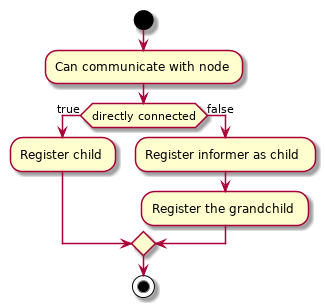
\includegraphics[width=.45\linewidth]{UML/out/Communication/activity/contactgevonden/contactgevonden.png}\end{center}
	\caption{Activity diagram vinden pad tot adres}
	\label{fig:communication:routeringtechniek:gevonde}
\end{figure}

Op het moment dat er contact gelegd is dan wordt er gekeken of dit direct contact was of dat er een aangesloten node een nieuw contact heeft gevonden. Als het direct contact was komt er een nieuwe route aftakking door het toevoegen van een kind van de node.
Als er indirect een nieuw contact wordt gevonden dan wordt de gene die dit aangeeft geregistreerd als nieuw punt wanneer die nog onbekend was. Vervolgens wordt aan het adres die gevonden is toegevoegd aan de set van de gene die de vondst aangeeft.

\subsection{Ontwerpkeuzes gemaakt voor het communicatie component}
\label{DetailedDesign:Communicatie:ontwerkeuzes}
In het volgende stuk worden de keuzes gemaakt voor het component toegelicht.

%\subsubsection{}

\section{Design Sub-Systeem gazebo}
\label{DetailedDesign:MeshNetwerk}
Het sub syteem gazebo is het component die verantwoordelijk is voor de simulatie van de drones. 
Het is zowel verantwoordelijk voor het initialiseren van de virtuele hardware als aan elkaar koppelen van deze hardware.
Hoewel het nu nog niet van toepassing is zal gazebo uiteindelijk ook verantwoordelijk voor het toepassen van physics op de virutele drones. 


\subsection{Component Diagram}
\label{DetailedDesign:MeshNetwerk:ComponentDiagram}
\begin{figure}[H]
	\begin{center}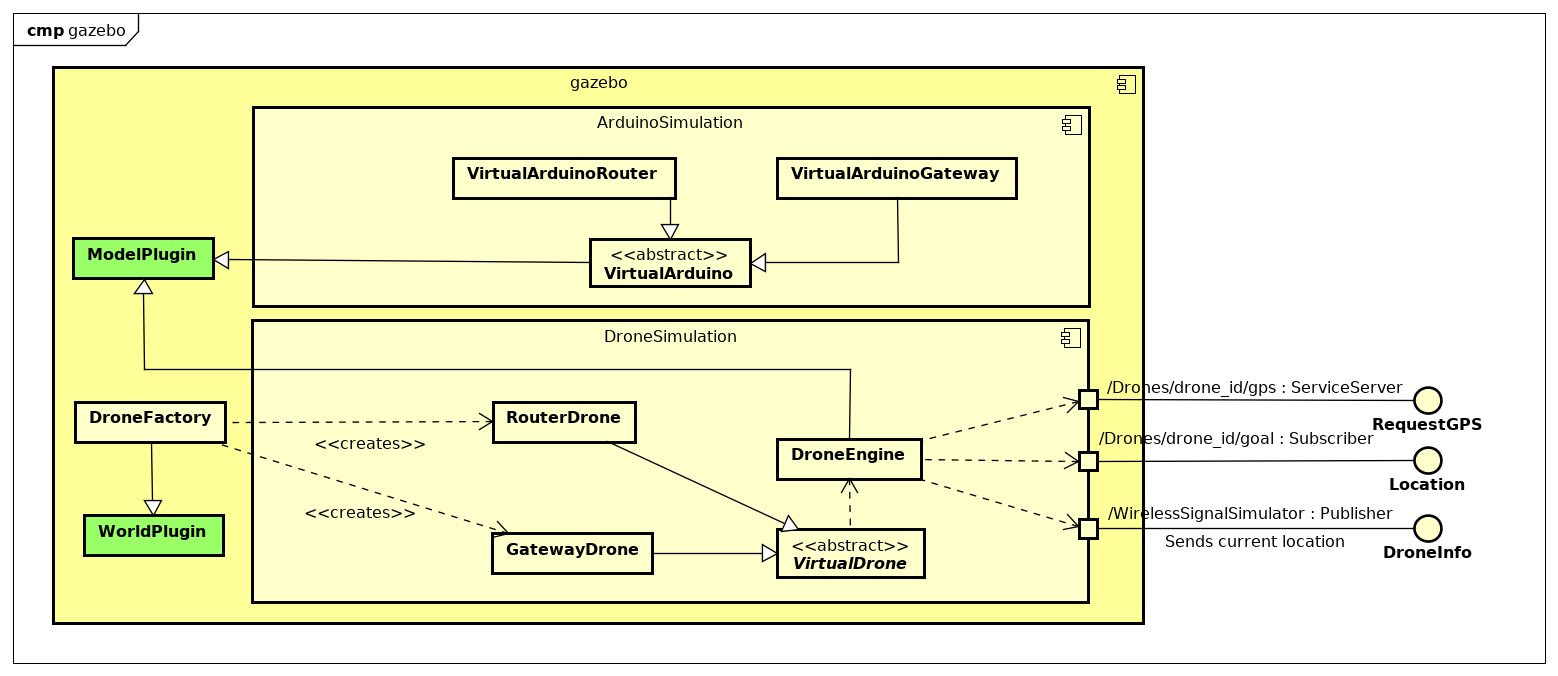
\includegraphics[width=\linewidth]{Afbeeldingen/gazeboComponentDiagram.png}\end{center}
	\caption{component diagram gazebo}
	\label{fig:component:gazebo}
\end{figure}

%NAMESPACE GAZEBO
\subsubsection{RaspberryPiSimulation}
\label{architectural:subcomponenten:RaspberryPiSimulation}
In de dit component wordt een Raspberry Pi gesimuleerd, deze simulatie is puur functioneel.
Het heeft geen effect op de clock snelheid deze is gelijk aan de computer waarop de software draait. 

\subsubsection{VirtualRaspberryPi}
\label{architectural:subcomponenten:VirtualRaspberryPi}
Dit abstracte component wordt gebruikt ter generalisatie van een Raspberry Pi
Omdat deze Raspberry Pi altijd wordt toegevoegd aan een ander model erft dit component over van modelplugin.    

\subsubsection{VirtualRaspberryPiRouter}
\label{architectural:subcomponenten:VirtualRaspberryPiRouter}
Deze \nameref{architectural:subcomponenten:VirtualRaspberryPi} is voorzien van een applicatie die de Raspberry Pi zich laat gedragen als in router in het meshnetwerk. 

\subsubsection{VirtualRaspberryPiGateway}
\label{architectural:subcomponenten:VirtualRaspberryPiGateway}
Deze \nameref{architectural:subcomponenten:VirtualRaspberryPi} is voorzien van een applicatie die de Raspberry Pi zich laat gedragen als in gateway in het meshnetwerk. 


\subsubsection{DroneSimulation}
\label{architectural:subcomponenten:DroneSimulation}
Dit component is verantwoordelijk voor het simuleren van drones. 

\subsubsection{DroneEngine}
\label{architectural:subcomponenten:DroneEngine}
Elke \nameref{architectural:subcomponenten:VirtualDrone} is voorzien deze drone engine. 
Dit component maakt het mogelijk voor een drone om zich in een rechte lijn door lucht zich te verplaatsen waarbij het opstijgen en de landing verticaal wordt uitgevoerd.
Daarnaast biedt dit component via een rosservice het deel van de interface \nameref{architectural:interfaces:IDroneEngine} aan om de huidige locatie op te vragen.
Via een rostopic kan er een doel gestuurd gestuurd worden om het andere deel van de net genoemde interface te voorzien.
Tenslotte stuurt dit component bij elke verplaatsing de huidige locatie door naar de \nameref{architectural:subcomponenten:WirelessSignalSimulator}. 

\subsubsection{VirtualDrone}
\label{architectural:subcomponenten:VirtualDrone}
Een virtuele drone is een abstract component die alle variabelen bevat die nodig zijn om een drone in de wereld te injecteren. Deze variabelen betreffen een drone id, locatie en verwijzing naar de gazebo wereld. 

\subsubsection{GatewayDrone}
\label{architectural:subcomponenten:GatewayDrone}
Deze drone is een \nameref{architectural:subcomponenten:VirtualDrone} die in de sdf omschrijving wordt voorzien van een \nameref{architectural:subcomponenten:VirtualRaspberryPiGateway} plugin. 
\subsubsection{RouterDrone}
\label{architectural:subcomponenten:RouterDrone}
Deze drone is een \nameref{architectural:subcomponenten:VirtualDrone} die in de sdf omschrijving wordt voorzien van een \nameref{architectural:subcomponenten:VirtualRaspberryPiRouter} plugin. 

\subsubsection{DroneFactory}
\label{architectural:subcomponenten:DroneFactory}
Dit component is verantwoordelijk voor het produceren van drones. Het is een WorldPlugin die aan de hand van meegegeven parameters gateway en router drones aanmaakt. Een dronefactory is afhankelijk van de SDF omschrijving in een .world bestand die er in factory.world er als volgt uitziet:

\begin{lstlisting}
<plugin name="DroneFactory" filename="libDroneFactory.so">
	<amountOfRouterDrones>17</amountOfRouterDrones>
	<amountOfGatewayDrones>1</amountOfGatewayDrones>
	<Debug>1</Debug>
</plugin>
\end{lstlisting}

\paragraph{amountOfRouterDrones} Hiermee wordt het aantal in te laden router drones bepaald.
 
\paragraph{amountOfRouterDrones} Hiermee wordt het aantal in te laden gateway drones bepaald.

\paragraph{Debug} Deze boolean bepaalt of de drones wel of geen debuging topic zullen hebben.

\subsection{Interfaces}
\label{DetailedDesign:MeshNetwerk:interfaces}
In de vorm van ros transport types voldoet het gazebo component aan extern aangeboden interfaces.
Door gebruik te maken van een ServiceServer \nameref{architectural:ros:service:RequestGPS} en een subscriber op het topic \nameref{architectural:ros:topic:Location} die samen de functionaliteit bieden benodigd voor de interface \nameref{architectural:interfaces:IDroneEngine}. 
Door informatie te publiceren op het topic \nameref{architectural:ros:topic:DroneInfo} biedt het informatie per drone aan over locaties.

\subsubsection{/Drones/drone\textunderscore id/gps}
\label{DetailedDesign:MeshNetwerk:interfaces:requestgps}

Elke drone engine maakt een service aan met de naam "\slash Drones/drone\textunderscore id/gps"	waarbij de drone\textunderscore id een variabele is.
De structuur van de service ziet er als volgt uit.
\begin{lstlisting}
---
float32 latitude
float32 longitude
int16 height
\end{lstlisting}

Deze service heeft geen parameters waaraan voldaan moet worden. 
Als response geeft het de huidige locatie terug van de drone.

\subsubsection{/Drones/drone\textunderscore id/goal}
\label{DetailedDesign:MeshNetwerk:interfaces:location}

Door te luisteren naar dit topic is het mogelijk om doelen te sturen naar de drone. 
Dit gebeurd door Location berichten te sturen naar de drone welke de volgende structuur hebben.

\begin{lstlisting}
float32 latitude
float32 longitude
int16 height
\end{lstlisting}

Bij ontvangst stelt de DroneEngine de ontvangen locatie in als doel.

\subsubsection{\slash WirelessSignalSimulator\slash}
\label{DetailedDesign:MeshNetwerk:interfaces:droneinfo}
Tenslotte publiceert de drone informatie op dit topic voor de \nameref{architectural:subcomponenten:WirelessSignalSimulator}
Hiervoor gebruikt het het bericht DroneInfo die de volgende structuur heeft:

\begin{lstlisting}
uint8 nodeID
float32[3] position
string sub
bool on
\end{lstlisting}

De DroneEngine vult alleen de informatie uit het bericht die hij bekend heeft.
Dit houdt dus in dat het ID van de drone verstuurd wordt en de positie waar die op dit moment is.

\subsection{Sequence Diagrams}
\label{DetailedDesign:MeshNetwerk:sequence}
In de onderstaande diagrammen wordt de sequentie weergeven die uitgevoerd wordt in het component gazebo. 
Eerst worden de virtuele RaspberryPi's behandeld waarna de dronefactory vervolgens aan bod komt. 

\paragraph{Opstarten virtuele RaspberryPi}
\label{DetailedDesign:MeshNetwerk:sequence:startenRaspberryPi}
Doordat er maar een minimaal verschil zit tussen het opstarten van een virtuele router Raspberry Pi en een virtuele gateway Raspberry Pi worden deze samen behandeld.


\begin{figure}[H]
	\begin{center}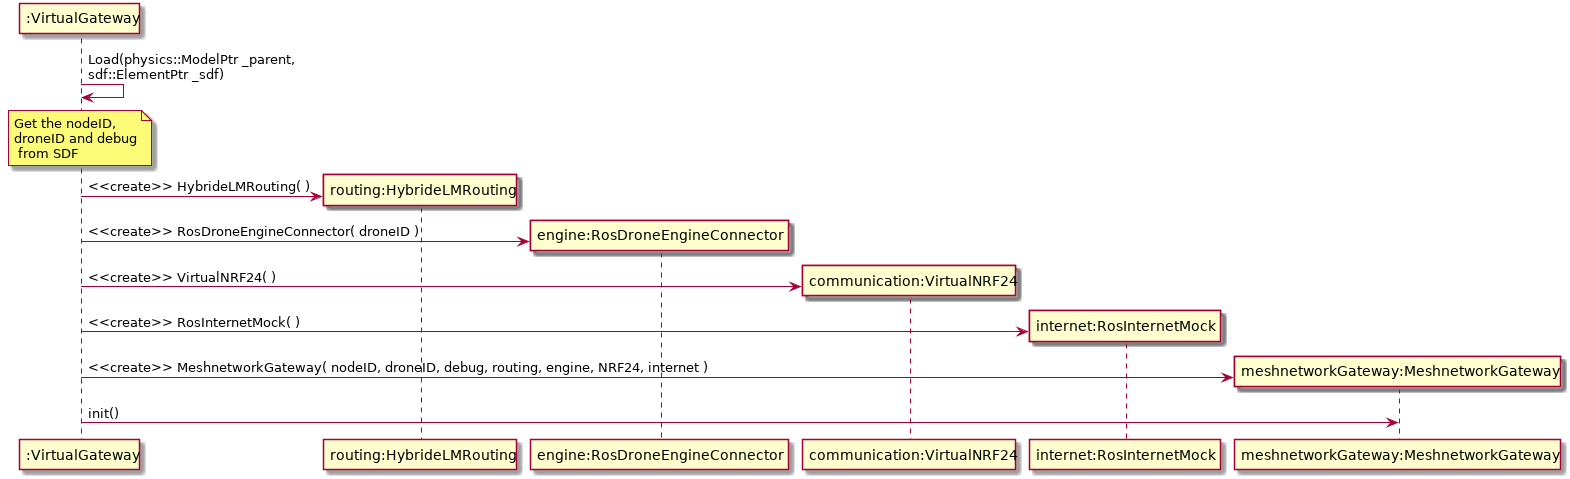
\includegraphics[width=.90\linewidth]{UML/out/DroneSimulation/Sequence/VirtualGateway/VirtualGateway.png}\end{center}
	\caption{Sequence diagram initialiseren van een virtuele gateway Raspberry Pi}
	\label{fig:communication:MeshNetwerk:sequence:gatewayRaspberryPi}
\end{figure}

\begin{figure}[H]
	\begin{center}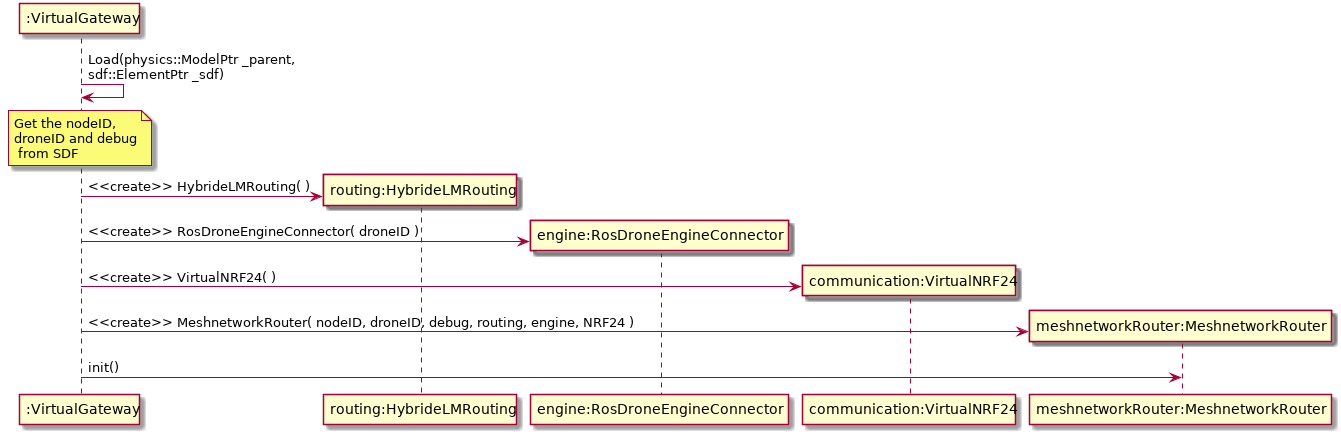
\includegraphics[width=.90\linewidth]{UML/out/DroneSimulation/Sequence/VirtualRouter/VirtualRouter.png}\end{center}
	\caption{Sequence diagram initialiseren van een virtuele gateway Raspberry Pi}
	\label{fig:communication:MeshNetwerk:sequence:routerRaspberryPi}
\end{figure}

In beiden gevallen begint het opstarten van de virtuele Raspberry Pi met het uitlezen van SDF waardes waar de parameters NodeID, DroneID en debug uit gehaald wordt.
Vervolgens wordt er een instantie van de routeringstechniek, DroneEngine connector, Virtuele NRF24 aangemaakt.
In het geval van de gateway wordt er ook nog een RosInternetMock aangemaakt.

Tenslotte wordt er een meshnetwerk gateway of router aangemaakt die een verwijzing meekrijgt naar de zojuist aangemaakte componenten.
Als laatste stap wordt het meshnetwerkcomponent aangeroepen om te starten met een init functie.

\paragraph{Drone factory}
\label{DetailedDesign:MeshNetwerk:sequence:dronefactory}
In de volgende sequentie wordt het opstarten van een dronefactory behandeld.   

\begin{figure}[H]
	\begin{center}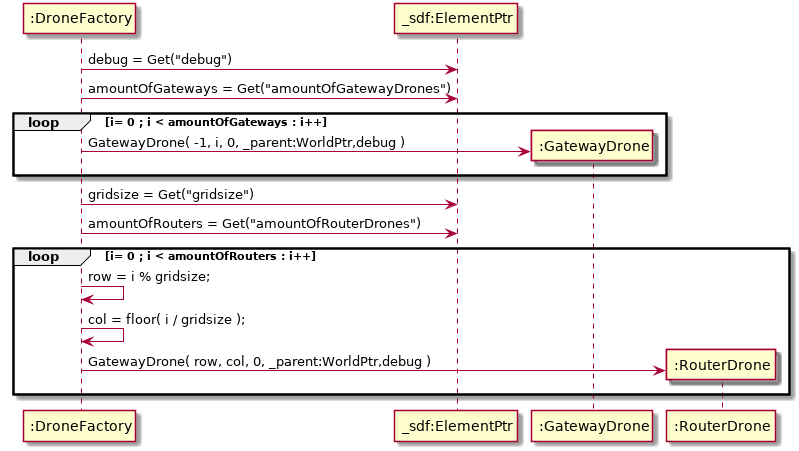
\includegraphics[width=.90\linewidth]{UML/out/DroneSimulation/Sequence/DroneFactory/DroneFactory.png}\end{center}
	\caption{Sequence diagram over het opstarten van een dronefactory}
	\label{fig:communication:MeshNetwerk:sequence:dronefactory}
\end{figure}

Bij het opstarten van een drone factory wordt de sdf geraadpleegd hoeveel gateway aangemaakt moeten worden. 
Vervolgens zal de factory per gateway een instantie aanmaken die zichzelf via een sdf omschrijving injecteert in gazebo.
Deze sdf omschrijving wordt later in deze paragraaf verder toegelicht, tegelijk met die van een router drone.

Nadat de factory alle gateway drones heeft gemaakt worden de router drones gemaakt.
Voordat hij de drones aanmaakt raadpleegt de factory het sdf bestand nogmaal om de variabele gridsize in te stellen.
Gridsize bepaalt hoe breed elke kolom maximaal mag zijn

Nadat de RouterDrones zijn aangemaakt is het factory programma klaar en zal het niks meer uitvoeren tijdens de simulatie.

\subparagraph{SDF omschrijvingen drones}
\label{DetailedDesign:MeshNetwerk:sequence:dronefactory:droneomschrijvingen}
Een drone inject bij de constructor een SDF omschrijving van zichzelf in gazebo.
Deze omschrijvingen worden nu behandeld.

Een sdf omschfrijving van een router drone ziet er als volgt uit:
\begin{lstlisting}
<sdf version ='1.6'>
 <model name ='router_drone'>
  <static>1</static>
  <pose>x y z 0 0 0</pose>
  <link name ='link'>
   <inertial>
    <pose>x y z 0 0 0</pose>
   </inertial>
   <collision name ='collision'>
    <geometry>
     <box><size>0.5 0.5 0.5</size></box>
    </geometry>
   </collision>
   <visual name ='visual'>
    <geometry>
     <box><size>0.5 0.5 0.5</size></box>
    </geometry>
    <material>
    <script>
     <uri>file://media/materials/scripts/gazebo.material</uri>
     <name>Gazebo/Green</name>
    </script>
    </material>
   </visual>
  </link>
  <plugin name="MeshnetworkRouter" filename="libMeshnetworkRouter.so">
   <DroneID> droneID </DroneID>
   <nodeID> droneID </nodeID>
   <Debug> debug </Debug>
  </plugin>
  <plugin filename = 'libDroneEngine.so' name ='DroneEngine'>
   <DroneID> droneID </DroneID> 
  </plugin>
 </model >
</sdf>"
\end{lstlisting} 

Een sdf omschfrijving van een gateway drone ziet er bijna hetzelfde uit behalve dat deze aanspraak maakt op de plugin "MeshnetworkGateway"\ in plaats van "MeshnetworkRouter".  En de gebruikte kleur paars is in plaats van groen.

Belangrijke punten uit deze omschrijving zijn:

\textbf{static:} Door deze op waar te zetten wordt de drone niet meegenomen in de physics engine.

\textbf{x y z: } Deze worden gebruikt voor het positioneren van de drone.

\textbf{Material:} Hierin wordt een script aangeroepen om een kleur toe te wijzen aan de drone.

\textbf{plugin name="MeshnetworkRouter" filename="libMeshnetworkRouter.so"} Deze plugin zorgt ervoor dat een drone voorzien wordt van een \nameref{architectural:subcomponenten:VirtualRaspberryPiRouter}.

\textbf{plugin name="MeshnetworkGateway" filename="libMeshnetworkGateway.so"} Deze plugin zorgt ervoor dat een drone voorzien wordt van een \nameref{architectural:subcomponenten:VirtualRaspberryPiGateway}. Deze plugin is niet zichtbaar in het bovenstaande SDF voorbeeld maar wordt wel gebruikt in het sdf format voor een gateway 

\textbf{plugin filename = 'libDroneEngine.so' name ='DroneEngine'} Deze plugin zorgt ervoor dat een drone wordt voorzien van eem \nameref{architectural:subcomponenten:DroneEngine}


\textbf{DroneID:} Dit zal het ID zijn van de drone zelf en wordt aan de motor gekoppeld, deze moet uniek zijn in het programma. Anders zullen er meerdere drones aangestuurd worden.

\textbf{nodeID:} Dit zal het ID zijn van het aangesloten netwerkcomponent. Ook deze moet uniek zijn in de huidige implementatie. 

\textbf{Debug:} Op het moment dat deze aanstaat zal een netwerkcomponent zijn debug stand gebruiken.



\subsection{Activity Diagrammen}
\label{DetailedDesign:MeshNetwerk:activity}


\paragraph{DroneEngine applicatie}
\label{DetailedDesign:MeshNetwerk:Activity:initaliserenDrone}
Elke drone is voorzien van een DroneEngine, dit component zorgt ervoor dat de drone in de simulatie kan voortbewegen op basis van doelen.
Daarnaast biedt het de optie om de locatie van een drone op te vragen om zo een abstracte versie van een GPS na te bootsen.
\begin{figure}[H]
	\begin{center}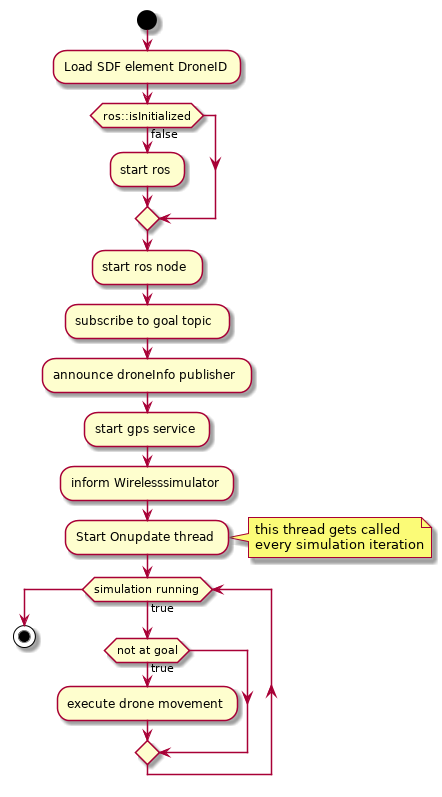
\includegraphics[width=.45\linewidth]{UML/out/DroneSimulation/Activity/DroneEngine/DroneEngine.png}\end{center}
	\caption{Activity diagram initialiseren van de DroneEngine}
	\label{fig:communication:MeshNetwerk:Activity:initialiserenDrone}
\end{figure}

Op het moment dat een DroneEngine gestart wordt is het ophalen van de DroneID  het eerste wat het component doet.
Vervolgens controleert het component of ROS al gestart is.
Wanneer deze nog niet gestart is wordt deze alsnog opgestart.
Vervolgens wordt er een eigen rosnode gecreëerd.
Deze rosnode wordt vervolgens gebruikt om te luisteren naar het topic waarvan de drone zijn doel locatie binnen krijgt.
Hierna start de node een topic met droneinformatie waar de locatie van de drone en het id in staat.
Vervolgens wordt er ook de gps service gestart.
Nu dit allemaal opgestart is wordt er een bericht gestuurd naar de wireless simulator met de huidige drone informatie.

Om het initialiseren af te maken wordt er tenslotte een thread gestart die elke simulatie cycle wordt aangeroepen.
Deze thread controleert per cycle of de drone op zijn huidige doel is.
Als deze dat niet is wordt er een functie aangeroepen om de drone naar zijn doel toe te laten bewegen.
Hoe deze animatie werkt wordt in het hierop volgende activity diagram uitgelegd   


\paragraph{Uitvoeren van een beweging van de drone}
\label{DetailedDesign:MeshNetwerk:Activity:AnimatieDrone}
Voor het uitvoeren van een beweging maakt de drone gebruik van een animiatie. 
Dit is mogelijk omdat de DroneEngine een modelplugin is waardoor het aanspraak kan maken op de pose van de aangesloten drone.
  

\begin{figure}[H]
	\begin{center}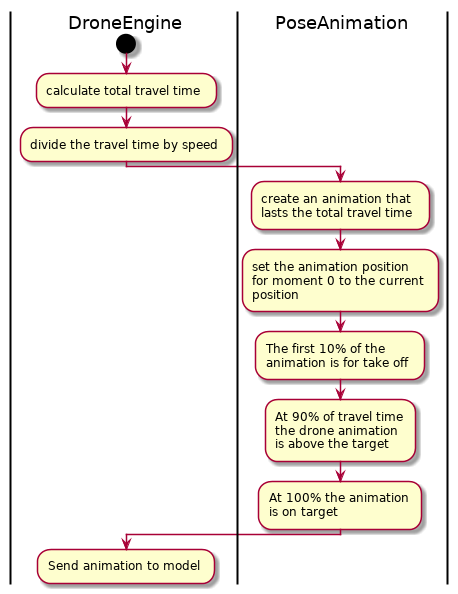
\includegraphics[width=.45\linewidth]{UML/out/DroneSimulation/Activity/DroneMovement/DroneMovement.png}\end{center}
	\caption{Activity diagram vinden pad tot adres}
	\label{fig:communication:MeshNetwerk:Activity:AnimatieDrone}
\end{figure}

Op het moment dat er een beweging verzocht wordt begint de drone met het berekenen wat de directe afstand is tussen de drone en het doel.
Zodra de afstand berekend is wordt de afstand gedeeld door de snelheid waardoor er een tijd ontstaat die de beweging zal kosten.

De eerste stap van de animatie is het instellen waar de animatie begint op tijdstip 0, in deze implementatie is dat op de locatie waar de drone al is.
Vervolgens moet de drone opstijgen dit duurt 10 procent van de totale tijd die de drone beweegt.
De hoogte van het opstijgen heeft een verband met afstand dit is namelijk de helft hiervan.
Vervolgens wordt op 90 procent van de animatie een doel ingestelt om weer op dezelfde hoogte boven het doel te hangen.
Tenslotte moet de animatie bij 100 procent landen op het ingestelde doel.

Als deze volledige animatie is ingesteld wordt dit verstuurd naar het model om uit te voeren.    
 

\subsection{Ontwerpkeuzes gemaakt voor het gazebo component}
\label{DetailedDesign:gazebo:ontwerkeuzes}
In het volgende stuk worden de keuzes gemaakt voor het component toegelicht.


\section{Design Sub-System ros}
\label{DetailedDesign:WirelessSimulatie}
Het volgende gedeelte zal gaan over het subcomponent ros. Het component is verantwoordelijk voor het simuleren van alle vormen van communicatie die gebruikt worden in het meshnetwerk. Het simuleert een NRF24 inclusief de draadloze communicatie.

\subsection{Component Diagram}
\label{DetailedDesign:ros:ComponentDiagram}
\begin{figure}[H]
	\begin{center}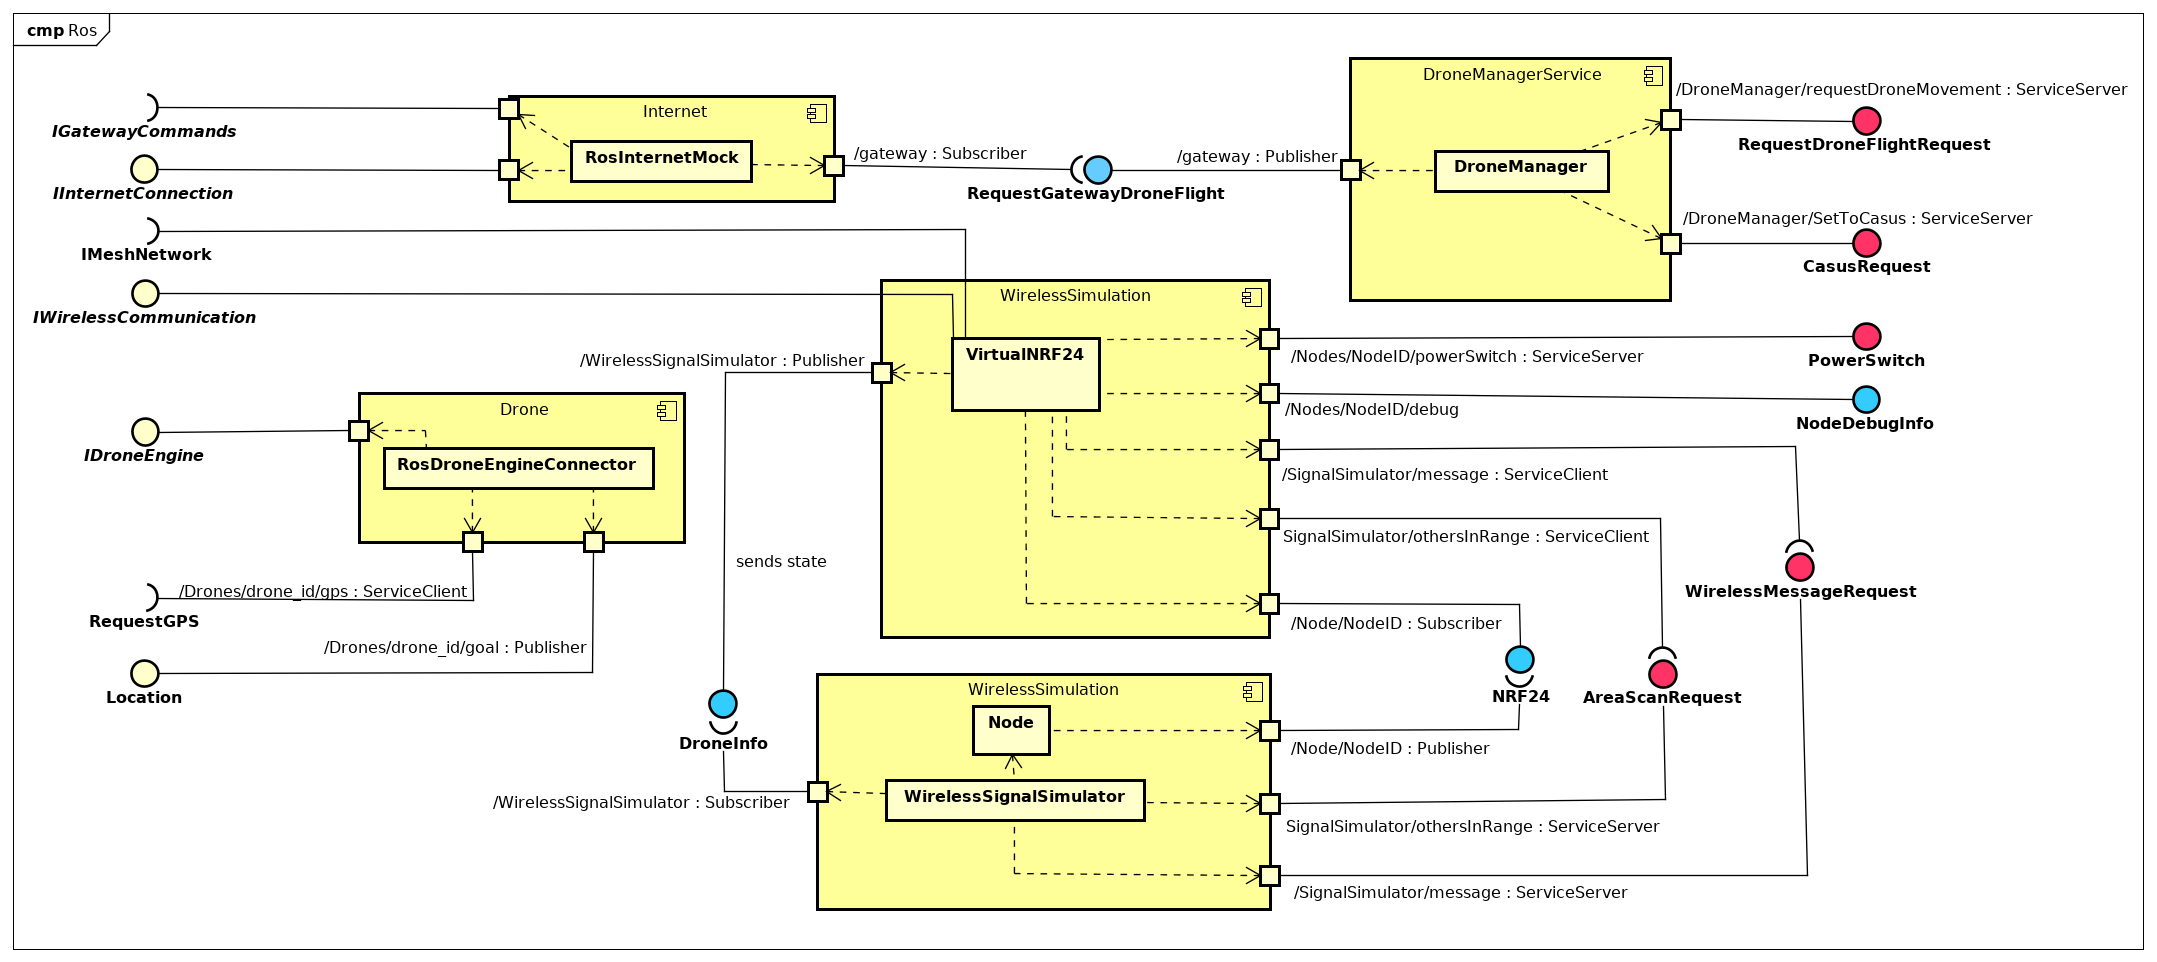
\includegraphics[width=\linewidth]{Afbeeldingen/rosComponentDiagram.png}\end{center}
	\caption{component diagram ros}
	\label{fig:component:ros}
\end{figure}

%NAMESPACE Ros
\subsubsection{RosDroneEngineConnector}
\label{architectural:subcomponenten:RosDroneEngineConnector}
Dit component is een adapter tussen de \nameref{architectural:subcomponenten:DroneEngine} en de interface \nameref{architectural:interfaces:IDroneEngine}. Die het mogelijk maakt om ros te gebruiken om aanspraak te maken op de virtuele drone.

\subsubsection{DroneManagerService}
\label{architectural:subcomponenten:DroneManagerService}
Dit component is de toegangspoort voor de ontwikkelaar tot de \nameref{architectural:subcomponenten:MeshnetworkGateway}.
Op dit moment is het component alleen geschikt om verplaatsingverzoeken te versturen via de gateway naar de Drones.
Hiervoor biedt het twee interfaces in de vorm van rosservices aan waarbij er een voor locaties is en de ander voor casussen. 

\subsubsection{DroneManager}
\label{architectural:subcomponenten:DroneManager}
Dit subcomponent realiseert de rosservices en publiceert verplaatsingverzoeken naar de gateways.  

\subsubsection{RosInternetMock}
\label{architectural:subcomponenten:RosInternetMock}
Deze internetmock laat de \nameref{architectural:subcomponenten:DroneManager} zich voordoen als internetpunt zodat er geen daadwerkelijke TCP/IP implementatie hoeft worden gemaakt 
\subsubsection{WirelessSimulation}
\label{architectural:subcomponenten:WirelessSimulation}
Het WirelessSimulation component is verantwoordelijk voor het simuleren van de NRF24 en het draadloze signaal hiervan. 
\subsubsection{WirelessSignalSimulator}
\label{architectural:subcomponenten:WirelessSignalSimulator}
Deze simulator bepaald of twee nodes met elkaar mogen communiceren. Het doet dit op basis van informatie die het continue ontvangt via het drone informatie topic. 
\subsubsection{Node}
\label{architectural:subcomponenten:Node}
Dit component wordt alleen gebruikt door de \nameref{architectural:subcomponenten:WirelessSignalSimulator} om te registreren welke Nodes bestaan, waar ze zijn en naar welk topic ze luisteren.
\subsubsection{VirtualNRF24}
\label{architectural:subcomponenten:VirtualNRF24}
Dit component is de virtuele versie van de NRF24, het is in staat om payloads te verwerken van 32 byte.
Deze kan de NRF24 naar een direct adres versturen of zenden naar alle NRF24 nodes binnen bereik.

\subsubsection{Extern aangeboden interfaces}
\label{DetailedDesign:ros:extern:interfaces}

\paragraph{IInternetConnection}
\label{DetailedDesign:ros:extern:interfaces:IInternetConnection}
Deze interface wordt aangeboden door \nameref{architectural:subcomponenten:RosInternetMock} biedt daarmee de optie om een internet verbinding op te zetten. 
 
\begin{lstlisting}
void Connect(IGatewayCommands* IGC) 
void Disconnect( )
\end{lstlisting}

\subparagraph{Connect} 
\label{DetailedDesign:ros:extern:interfaces:IInternetConnection:Connect}
Deze functie wordt aangeroepen om een verbinding op te zetten.
Als parameter wordt een verwijzing naar een aangeboden interface verwacht waar de internetconnectie gebruik van mag maken om commando's het netwerk in te sturen. 

\textbf{\textit{preconditie:}} Component die een internetverbinding wil maken kan de interface \nameref{architectural:interfaces:IGatewayCommands} aanbieden.

\textbf{\textit{postconditie:}} Er is een externe verbinding buiten het meshnetwerk opgezet geschikt om commando's het netwerk in te sturen.

\subparagraph{Disconnect} 
\label{DetailedDesign:ros:extern:interfaces:IInternetConnection:Disconnect}
Deze functie wordt aangeroepen om een internet verbinding te verbreken.

\textbf{\textit{preconditie:}} Er is geen postconditie aan deze functie. 
Wanneer er nog geen verbinding bestond zal de uitkomst het zelfde blijven

\textbf{\textit{postconditie:}} Er bestaat geen internetverbinding meer. 

\paragraph{IWirelessCommunication}
\label{DetailedDesign:ros:extern:interfaces:IWirelessCommunication}
Deze interface wordt gebruikt om een draadloos communicatie middel aan te kunnen bieden.

\begin{lstlisting}
void StartAntenna(IMeshNetwork* IMN)
void StopAntenna( )
bool SendMessageTo(const uint8_t* msg)
void BroadcastMessage(const uint8_t* msg)
void DebugingMode(IMeshDebugInfo* IMD, const bool on)
const bool On( )
\end{lstlisting}

\subparagraph{StartAntenna}
\label{DetailedDesign:ros:extern:interfaces:IWirelessCommunication:StartAntenna}
Deze functie wordt gebruikt om de antenne te starten. Het verwacht een pointer terug naar het MeshNetwerk waar de ontvangen berichten aangegeven kunnen worden.

\textbf{\textit{preconditie:}} De antenne is aangesloten op een een component die 32byte berichten kan verwerken

\textbf{\textit{postconditie:}} De antenne is gestart en klaar om berichten te ontvangen.

\subparagraph{StopAntenna}
\label{DetailedDesign:ros:extern:interfaces:IWirelessCommunication:StopAntenna}
Door het aanroepen van deze functie zal de aangesloten antenne stoppen.

\textbf{\textit{preconditie:}} Er is geen preconditie

\textbf{\textit{postconditie:}} De antenne is gestopt

\subparagraph{SendMessageTo}
\label{DetailedDesign:ros:extern:interfaces:IWirelessCommunication:SendMessageTo}
Deze functie verwacht een verwijzing naar een 32 byte array die vervolgens verstuurd zal worden

\textbf{\textit{preconditie:}}  Er is een bericht opgesteld om verstuurd te worden

\textbf{\textit{postconditie:}} Het bericht is verstuurd naar de geadresseerde

\subparagraph{BroadcastMessage}
\label{DetailedDesign:ros:extern:interfaces:IWirelessCommunication:BroadcastMessage}
Deze functie zal een 32 byte bericht versturen op het algemene kanaal van de NRF24 waardoor dus elke node binnen bereik dit zal ontvangen

\textbf{\textit{preconditie:}} Er is een bericht opgesteld die naar iedereen in de buurt verstuurd zal worden.

\textbf{\textit{postconditie:}} Elke node binnen bereik van deze antenne heeft het bericht ontvangen.


\subparagraph{DebugingMode}
\label{DetailedDesign:ros:extern:interfaces:IWirelessCommunication:DebuggingMode}
Deze functie verwacht een verwijzing naar debuginformatie over het meshnetwerk zodat dit samen met debuginfo van de antenne zelf gepubliceerd kan worden.

\textbf{\textit{preconditie:}} De aanvrager van deze functie beschikt over de interface \nameref{architectural:interfaces:IMeshDebugInfo}.

\textbf{\textit{postconditie:}} Er wordt debuginformatie gepubliceerd



\paragraph{IDroneEngine}
\label{DetailedDesign:ros:extern:interfaces:IDroneEngine}
Deze interface wordt gebruikt om een drone aan te sturen en zijn locatie op te kunnen vragen. Hij wordt aangeboden door \nameref{architectural:subcomponenten:RosDroneEngineConnector}

\begin{lstlisting}
void setGoal(const float latitude, const float longitude, const float height)
const Vector3< float > getLocation( )
\end{lstlisting}

\subparagraph{SetGoal}
\label{DetailedDesign:ros:extern:interfaces:IDroneEngine:SetGoal}
De functie wordt gebruikt om een doel in te stellen voor de drone om zich naartoe te verplaatsen.

\textbf{\textit{preconditie:}} Er is geen preconditie voor deze functie 

\textbf{\textit{postconditie:}} Er is een doel ingesteld in de drone waarnaar hij zich moet verplaatsen


\subparagraph{getLocation}
\label{DetailedDesign:ros:extern:interfaces:IDroneEngine:getLocation}
Deze functie wordt gebruikt om de huidige locatie van een drone op te vragen er wordt een latitude, logitude en een height verwacht in de vorm van een Vector3.

\textbf{\textit{preconditie:}} De drone heeft kennis van zijn huidige locatie.

\textbf{\textit{postconditie:}} De huidige locatie van de drone is berekend en teruggegeven.

\subsubsection{Extern aangeboden ros interfaces}
\label{DetailedDesign:ros:extern:rosinterfaces}
Via rosservices en topic biedt het component ook externe functionaliteit en functies aan deze worden hieronder behandeld.

\paragraph{/Drone/drone\textunderscore id/goal}
\label{DetailedDesign:ros:extern:rosinterfaces:topic:goal}
De \nameref{architectural:subcomponenten:RosDroneEngineConnector} publiceert doelen voor de drone op dit topic.
De doelen worden gepubliceerd met een Location message welke de volgende structuur heeft.

\begin{lstlisting}
float32 latitude
float32 longitude
int16 height
\end{lstlisting}


\paragraph{/DroneManager/requestDroneMovement}
\label{DetailedDesign:ros:extern:rosinterfaces:service:requestDronemovement}

Deze service wordt aangeboden door de \nameref{architectural:subcomponenten:DroneManager} het biedt de service aan om verzoeken te sturen naar de gateway om locatieverplatsingen uit te voeren. Het maakt gebruik van het servicebericht RequestDroneFlight. De structuur van dit bericht is als volgt.

\begin{lstlisting}
uint8 ID
float32 latitude
float32 longitude
int16 height
---
uint8 status
\end{lstlisting}

\subparagraph{ID} Is de parameter die gebruikt wordt om de ID van de te verplaatsen drone aan te geven.
\subparagraph{latitude, longitude, height} Zijn de parameters die gebruikt worden op de gewenste locatie op te geven.
\subparagraph{status} Deze response geeft aan of het de manager is gelukt om het verzoek te versturen naar de gateway.


\textbf{\textit{preconditie:}} De drone manager is verbonden met een drone gateway 

\textbf{\textit{postconditie:}} Er is een bericht gestuurd naar de gateway met een verzoek om een locatie te veranderen

\paragraph{/DroneManager/SetToCasus}
\label{DetailedDesign:ros:extern:rosinterfaces:service:casus}
De service die hier aangeboden wordt is een functie om drones te verplaatsen naar een casus positie.
Om deze functie te gebruiken wordt een casus bericht verwacht deze heeft de volgende structuur.

\begin{lstlisting}
uint32 caseID
\end{lstlisting}

Er is op dit moment één casus geïmplementeerd uit het plan van aanpak.
Deze casus gebruikt 17 drones. 
Daarom kan er met caseID 0 alle drones naar die casus positie gezet worden en met 1 t/m 17 worden ze individueel naar deze positie gebracht.
Met casus 100 wordt er een grid gemaakt van 10 bij 10 drones wanneer er minder aanwezig zijn vullen ze plek 0 tot het aantal wat er is.   

\textbf{\textit{preconditie:}}  De drone manager is verbonden met een drone gateway 

\textbf{\textit{postconditie:}} Er zijn één of meerdere verplaatsingverzoeken verstuurd naar de gateway om de drones naar hun casus positie te zetten.

\paragraph{/Nodes/NodeID/powerSwitch}
\label{DetailedDesign:ros:extern:rosinterfaces:service:powerswitch}
Deze service wordt aangeboden door het component \nameref{architectural:subcomponenten:VirtualNRF24} en representeert een aan en uit knop voor een antenne.
De service maakt gebruikt van een PowerSwitch bericht die de volgende structuur kent:

\begin{lstlisting}
bool power
\end{lstlisting}

De boolean die in het bericht zit bepaald of de antenne aan of uit wordt gezet.

\textbf{\textit{preconditie:}}  Er is geen post conditie een NRF24 kan altijd aan of uit gezet worden.

\textbf{\textit{postconditie:}} De antenne is gezet in de opgegeven aan/uit staat.

\paragraph{/Nodes/NodeID/debug}
\label{DetailedDesign:ros:extern:rosinterfaces:topic:debug}

Het volgende topic wordt gepubliceerd om de ontwikkelaar van informatie te voorzien over de node en aangesloten antenne.
\nameref{architectural:subcomponenten:VirtualNRF24} is de aanbieder van dit topic.
Het bericht wat gepubliceerd wordt op dit topic is een NodeDebugInfo bericht die de volgende structuur heeft:
\begin{lstlisting}
uint8 nodeID
bool ConnectedWithGateway 
uint16 familySize
uint32 totalMessages
uint8 prefferedGateWay
bool on
uint8 hops
uint8 prefLoc
\end{lstlisting}

\subparagraph{nodeID} Het ID van die de antenne gebruikt 
\subparagraph{ConnectedWithGateway} boolean die aangeeft of de node een verbinding heeft met een gateway
\subparagraph{familySize} Het aantal nodes die de huidige node kent. Niet directe nodes kunnen dubbel voorkomen
\subparagraph{totalMessages} Het totaal aantal berichten die een node verstuurt heeft
\subparagraph{prefferedGateWay} Het ID van de gateway waar de node voorkeur voor heeft
\subparagraph{on} boolean die aangeeft of de antenne aan staat
\subparagraph{hops} Het aantal hops die een node nodig heeft om de gateway te bereiken
\subparagraph{prefLoc} Het ID van een andere node waar deze node voorkeur voor heeft om in nood naartoe te verplaatsen. 

\subsubsection{Intern aangeboden ros interfaces}
\label{DetailedDesign:ros:intern:rosinterfaces}

\paragraph{/gateway}
\label{DetailedDesign:ros:intern:rosinterfaces:topic:gateway}
Het gateway topic is de verbinding tussen de \nameref{architectural:subcomponenten:DroneManager} en de \nameref{architectural:subcomponenten:RosInternetMock}.
Omdat er op dit moment alleen ondersteuning is voor verzoeken tot het verplaatsen van een wordt er gebruik gemaakt van het bericht RequestGatewayDroneflight.
Dit bericht heeft de volgende samenstelling:

\begin{lstlisting}
uint8 ID
float32 latitude
float32 longitude
int16 height
\end{lstlisting}

\subparagraph{ID} Het ID wordt gebruikt om aan te geven welke drone zich moet verplaatsen.
\subparagraph{latitude, longitude, height} Zijn de parameters die gebruikt worden op de gewenste locatie op te geven.

\paragraph{/Node/NodeID}
\label{DetailedDesign:ros:intern:rosinterfaces:topic:node}
Elke \nameref{architectural:subcomponenten:VirtualNRF24} maakt dit topic aan waarbij NodeID slaat op het ID van de node. 
Dit topic wordt gebruikt om NRF24 berichten te ontvangen van andere virtuele nodes via de \nameref{architectural:subcomponenten:WirelessSignalSimulator}  
De berichten die over dit topic verzonden worden zijn NRF24 berichten die de volgende structuur hebben:

\begin{lstlisting} 
uint8[32] payload
\end{lstlisting}

\subparagraph{payload} Een NRF24 is in staat berichten te versturen van maximaal 32 byte daarom telt dit ook voor het virtuele NRF24 bericht.


\paragraph{/SignalSimulator/othersinRange}
\label{DetailedDesign:ros:intern:rosinterfaces:service:ss:range}
Deze service wordt aangeboden door de \nameref{architectural:subcomponenten:WirelessSignalSimulator}.
Het maakt het mogelijk voor een node om op te vragen wie er allemaal binnen bereik is.
Het opvragen gaat via het servicebericht AreaScan die er al volgt uit ziet:

\begin{lstlisting}
uint8 id
---
uint8[] near
\end{lstlisting}

\subparagraph{id} Deze parameter staat voor welke node gekeken moet worden wie er allemaal binnen bereik is
\subparagraph{near} Als response wordt er een vector terug geven met alle nodes die in buurt zijn.

\paragraph{/SignalSimulator/message}
\label{DetailedDesign:ros:intern:rosinterfaces:service:ss:message}
Om een bericht te kunnen versturen biedt de  \nameref{architectural:subcomponenten:WirelessSignalSimulator} een service aan. 
Deze service verstuurd een bericht met opgelegde regels of het mogelijk zou zijn om een bericht te kunnen versturen.
Het servicebericht wat gebruikt wordt is een WirelessMessage bericht die de volgende samenstelling heeft:

\begin{lstlisting}
uint8 from
uint8 to 
NRF24 message
---
bool succes
\end{lstlisting}

\subparagraph{from} Het ID van de node die het bericht wil versturen.
\subparagraph{to} Het ID van de node waaraan het bericht verstuurd wordt
\subparagraph{NRF24} Het bericht die verstuurd moet worden.


\paragraph{/WirelessSignalSimulator}
\label{DetailedDesign:ros:intern:rosinterfaces:topic:signalsimulator}
De \nameref{architectural:subcomponenten:WirelessSignalSimulator} is het component die luistert naar dit topic. 
De berichten die hierop gepubliceerd worden zijn essentieel voor de simulator.
Dit omdat uit de berichten gehaald kan worden welke virtuele antennes bestaan en op welke positie zij zich bevinden.
Deze informatie wordt gepubliceerd aan de hand van het berichttype DroneInfo die er als volgt uit ziet:

\begin{lstlisting}
uint8 nodeID
float32[3] position
string sub
bool on
\end{lstlisting}

\subparagraph{NodeID} Het ID van de node waar de informatie betrekking op heeft.
\subparagraph{position} De positie waar de node zich bevindt gevuld met de volgende array [longitude][latitude][height]
\subparagraph{sub} Dit is de naam van het topic waar de \nameref{architectural:subcomponenten:VirtualNRF24} op luistert.
\subparagraph{on} Deze boolean geeft aan of de antenne aan of uit staat.

\subsection{Sequence Diagrams}
\label{DetailedDesign:ros:sequence}

Binnen het ros component vindt veel communicatie tussen componenten plaats door het gebruik van de ros transport laag.
Hoe deze communicatie verloopt wordt beter toegelicht met de volgende componenten.

\subsubsection{Verzoek tot verplaatsing van een drone}
\label{DetailedDesign:ros:sequence:verplaatsingdrone}

Een dronemanager biedt de service aan om een verzoek te versturen om een drone te verplaatsen. 
De dronemanager doet dit door te communiceren met het \nameref{architectural:subcomponenten:RosInternetMock} component.
Deze werking staat hieronder uitgelegd.

\begin{figure}[H]
	\begin{center}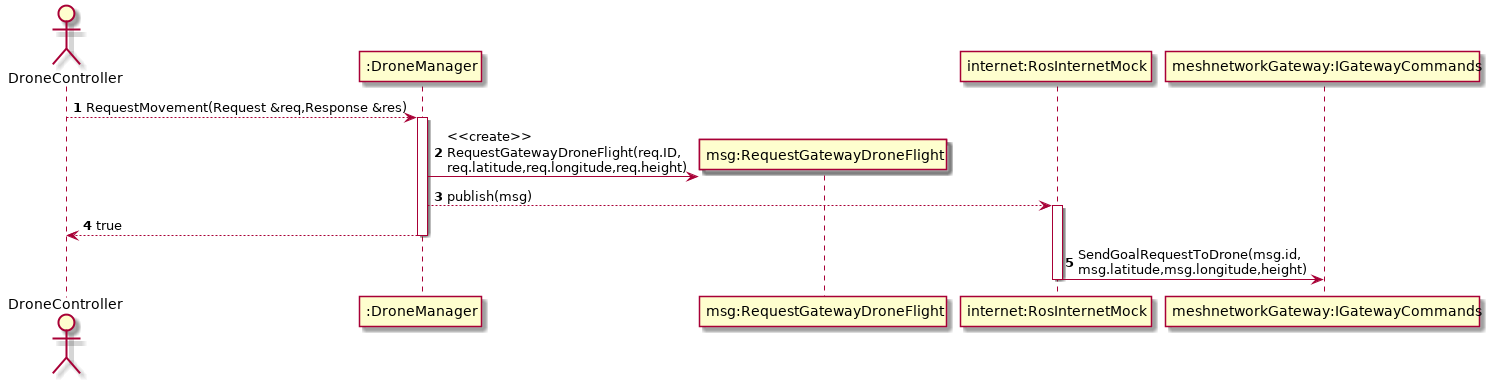
\includegraphics[width=.95\linewidth]{UML/out/ros/sequence/RequestDroneMovement/RequestDroneMovement.png}\end{center}
	\caption{Sequence diagram waarbij een DroneManager verzocht wordt een drone te verplaatsen}
	\label{fig:ros:sequence:sequence:verplaatsingdrone}
\end{figure}

Een actor kan een verzoek doen aan de drone manager om een drone te verplaatsen.
De drone manager verwacht hier een DroneFlightRequest bericht voor waar in staat wie er moet verplaatsen en waarheen.
Op basis van dit bericht maakt de DroneManager een RequestGatewayDroneFlight bericht aan en publiceert dit op het /gateway topic.
Elke RosInternetMock zal dit bericht ontvangen en versturen naar de \nameref{architectural:interfaces:IGatewayCommands} waar deze op aangesloten zit.
Per \nameref{architectural:subcomponenten:MeshnetworkGateway} bestaat er een RosInternetMock.

\subsubsection{Verzoek tot casus situatie}
\label{DetailedDesign:ros:sequence:casus}

Om het makkelijk te maken om situaties te testen heeft de drone manager een service die het aanbiedt om drone in bepaalde casus verdeling te zetten.

\begin{figure}[H]
	\begin{center}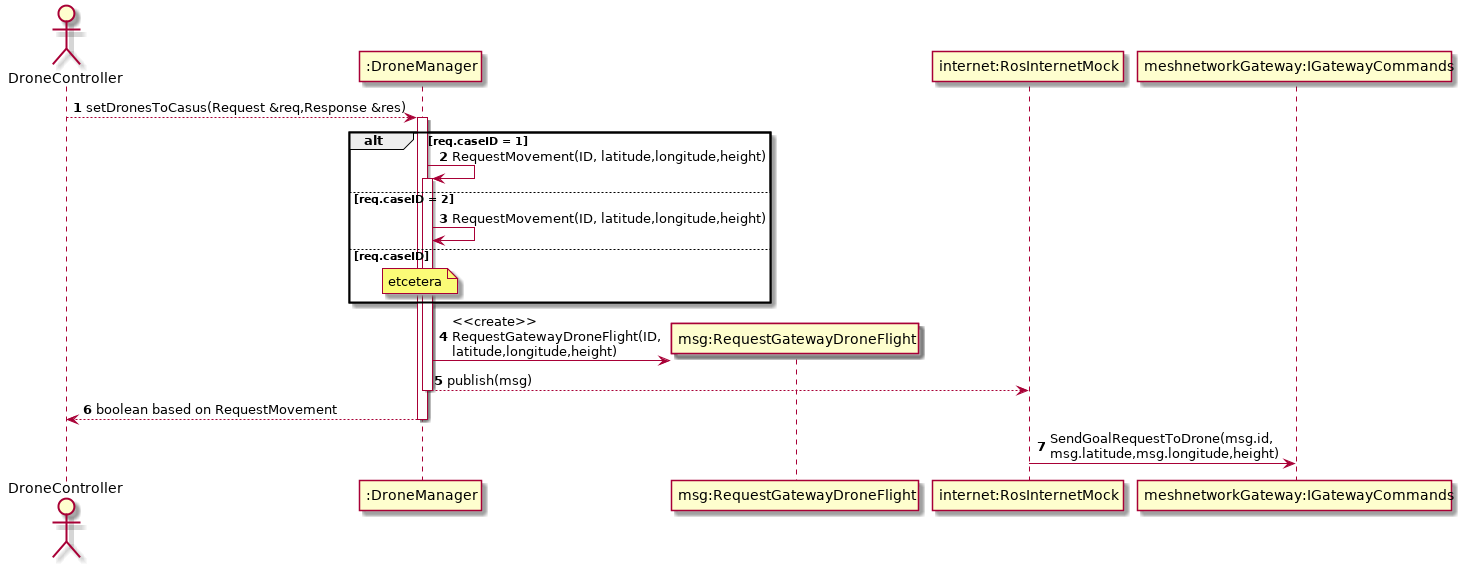
\includegraphics[width=.95\linewidth]{UML/out/ros/sequence/CasusRequest/CasusRequest.png}\end{center}
	\caption{Sequence diagram waarbij een DroneManager verzocht wordt een casus situatie te starten}
	\label{fig:ros:sequence:sequence:casus}
\end{figure}

De functie werkt grotendeels gelijk aan die van een verzoek tot een verplaatsing van een drone. 
Er wordt gebruik gemaakt van een switch case die reageert op het CaseID die gestuurd wordt.
Vervolgens kunnen daardoor een of meerdere RequestMovements aangeroepen worden om de drones te verzoeken te verplaatsen naar de casus positie. 

\subsubsection{Versturen bericht van VirtualNRF24 tot VirtualNRF24}
\label{DetailedDesign:ros:sequence:sendmessage}

Elk \nameref{architectural:subcomponenten:MeshnetworkComponent} is voorzien van een \nameref{architectural:subcomponenten:VirtualNRF24}.
Deze kunnen met elkaar communiceren maar om een draadloze situatie na te bootsen gebeurt dit via de \nameref{architectural:subcomponenten:WirelessSignalSimulator}.
Deze simulator bepaalt of dit mag op basis van onderlinge afstand en de aan/uit stand van de antenne.

\begin{figure}[H]
	\begin{center}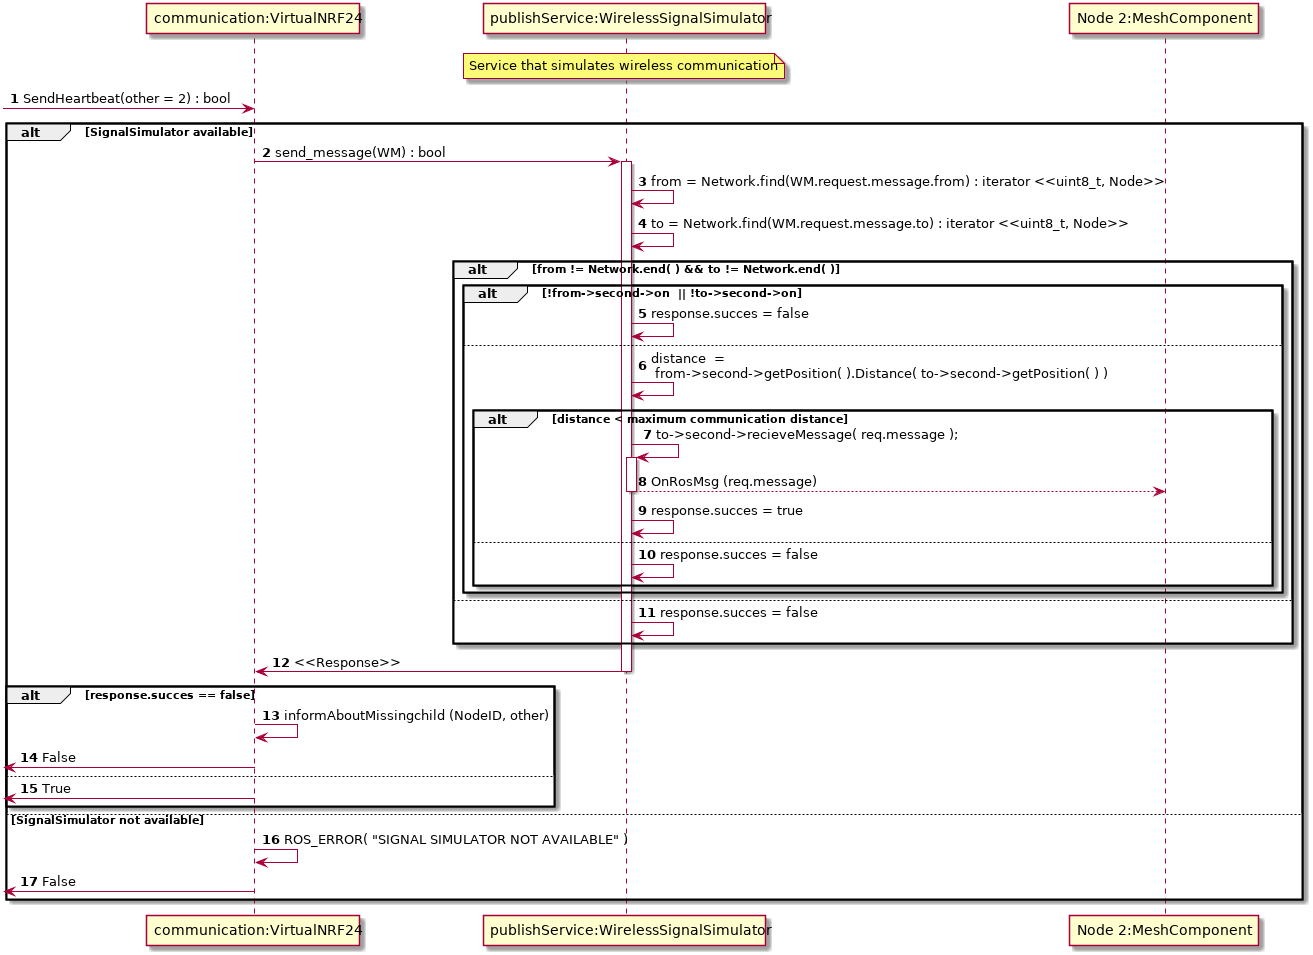
\includegraphics[width=\linewidth]{UML/out/ros/sequence/SendMessage/SendMessage.png}\end{center}
	\caption{Sequence diagram voor het versturen van een bericht van NRF24 tot NRF24}
	\label{fig:ros:sequence:sequence:sendmessage}
\end{figure}

Op het moment dat een \nameref{architectural:subcomponenten:VirtualNRF24} een verzoekt tot het versturen van een bericht ontvangt maakt het een WirelessMessage aan.
Hij stelt de zender en ontvanger van het bericht in en kopieert het bericht naar de payload van WirelessMessage.
Vervolgens wordt de service van de WirelessSignalSimulator voor het versturen van berichten aangeroepen om de WirelessMessage te versturen.
Als deze service niet beschikbaar is wordt er een ROS\textunderscore ERROR geprint zichtbaar in stap 21

Als de service wel beschikbaar is gaat deze als eerste kijken of hij de zender en ontvanger kent.
Vervolgens kijkt de WirelessSimulator of beide antennes aan staan
Wanneer één van de twee niet bekend is of er staat er één uit zal er een false als response terug gegeven worden.

Als dit niet het geval is zal er berekend worden wat de afstand is tussen de zender en de ontvanger.
Op het moment dat deze kleiner is dan de maximaal toegestaande communicatie afstand wordt het bericht verstuurd naar het topic waar de ontvangende \nameref{architectural:subcomponenten:VirtualNRF24} op luistert en wordt het succes van de response op true gezet.

De zendende NRF24 geeft de response van de \nameref{architectural:subcomponenten:WirelessSignalSimulator} terug om de functie te sluiten.

\subsubsection{Powerswitch service van de Virtuele NRF24}
\label{DetailedDesign:ros:sequence:powerswitch}

Elke \nameref{architectural:subcomponenten:VirtualNRF24} biedt een service aan om de NRF24 aan/uit te zetten.
Op het moment dat deze service wordt aangeroepen vindt het volgende plaats. 

\begin{figure}[H]
	\begin{center}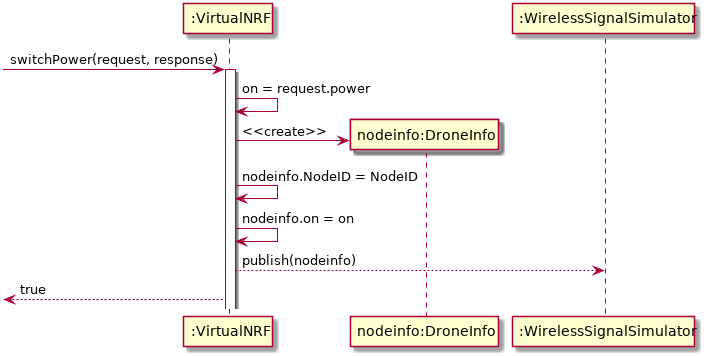
\includegraphics[width=.8\linewidth]{UML/out/ros/sequence/powerSwitch/powerSwitch.png}\end{center}
	\caption{Sequence diagram power switch Virtuele NRF24}
	\label{fig:ros:sequence:sequence:powerswitch}
\end{figure}

Zodra de functie aangeroepen wordt zet de antenne zijn staat gelijk aan die van de request.
Vervolgens maakt hij een DroneInfo bericht aan waar ingezet wordt wat de nieuwe staat en welk ID.
Dit bericht wordt tenslotte gepubliceerd naar de \nameref{architectural:subcomponenten:WirelessSignalSimulator}.



\subsubsection{Sturen doel naar drone}
\label{DetailedDesign:ros:sequence:sturendoelnaarengine}

De \nameref{architectural:subcomponenten:RosDroneEngineConnector} biedt in zijn aangeboden interface twee functies aan.
Een van die functies is het versturen van een doel naar de \nameref{architectural:subcomponenten:DroneEngine}. 

\begin{figure}[H]
	\begin{center}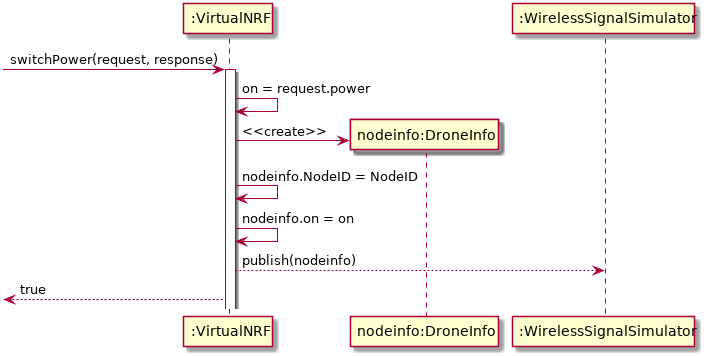
\includegraphics[width=.8\linewidth]{UML/out/ros/sequence/powerSwitch/powerSwitch.png}\end{center}
	\caption{Sequence diagram sturen doel naar de DroneEngine}
	\label{fig:ros:sequence:sequence:sturendoelnaarengine}
\end{figure}

Om een doel te versturen maakt de RosEngineConnector een Location bericht aan waarin de locatie staat waar de drone zich naartoe moet verplaatsen.
Deze publiceert hij vervolgens op het topic van de DroneEngine.

\subsubsection{Ophalen locatie van de drone}
\label{DetailedDesign:ros:sequence:ophalenlocatie}

De \nameref{architectural:subcomponenten:RosDroneEngineConnector} biedt in zijn aangeboden interface de functie aan om een locatie van een drone op te vragen. Dit werkt als volgt

\begin{figure}[H]
	\begin{center}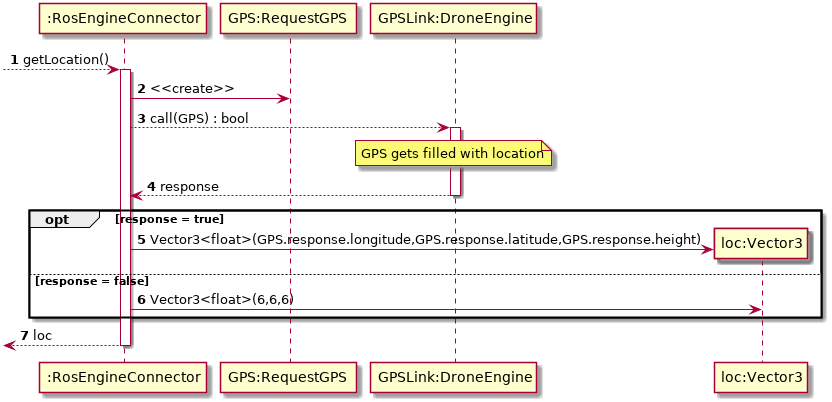
\includegraphics[width=.9\linewidth]{UML/out/ros/sequence/getLocation/getLocation.png}\end{center}
	\caption{Sequence diagram power switch Virtuele NRF24}
	\label{fig:ros:sequence:sequence:ophalenlocatie}
\end{figure}

Als er een verzoek om een locatie gemaakt wordt maakt de RosEngineConnector een RequestGPS bericht aan. 
Vervolgens gebruikt hij dit bericht in een servicecall naar de \nameref{architectural:subcomponenten:DroneEngine} die als response de locatie terug zal geven. 
Met deze waardes wordt een Vector3 aangemaakt welke vervolgens teruggegeven wordt.
Er is nog geen goede afhandeling wanneer de DroneEngine niet beschikbaar is voor nu wordt er locatie (6,6,6) teruggegeven.


\subsection{Activity Diagrammen}
%\subsection{Activity and State Diagrams}
\label{DetailedDesign:ros:activity}

\paragraph{Verwerken drone informatie WirelessSimulator}
\label{DetailedDesign:ros:Activity:droneinfo}
Er is een generiek topic van de wireless simulator waar zowel de \nameref{architectural:subcomponenten:DroneEngine} als de \nameref{architectural:subcomponenten:VirtualNRF24} informatie op posten. Om dit te scheiden neemt de WirelessSimulator de volgende stappen bij het ontvangen van een bericht. 
\begin{figure}[H]
	\begin{center}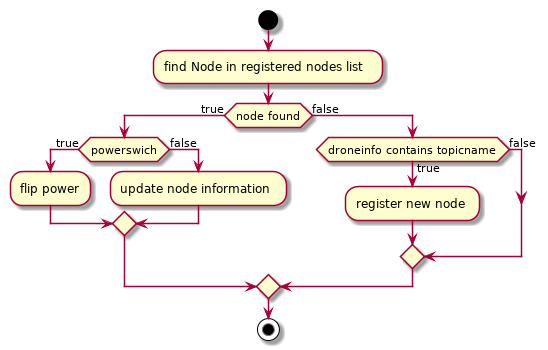
\includegraphics[width=.6\linewidth]{UML/out/ros/activity/processDroneInfo/processDroneInfo.png}\end{center}
	\caption{Activity diagram initialiseren van de DroneEngine}
	\label{fig:communication:MeshNetwerk:Activity:initialiserenDrone}
\end{figure}

Wanneer er een bericht ontvangen wordt met drone informatie kijkt de WirelessSimulator eerst of de node al bekend is bij hem.
Als deze nog niet bekend is kijkt de simulator of het bericht een string bevat met op welk topic de node luistert. 
Als niet in het bericht staat wordt de functie verlaten, wanneer dit wel zo wordt de node opgeslagen.

Wanneer het bericht van een bekende node af komt wordt er gekeken of er een power switch is.
Als dit zo is past de simulator ook de switch in zijn register voor die node aan zodat die weet in welke staat die staat.
Bij een bericht waar de stand van de power niet wisselt wordt de node zijn informatie bijgewerkt met de meest recente informatie.

\paragraph{Start antenne VirtualNRF24}
\label{DetailedDesign:ros:Activity:antenne}

Omdat er tijdens het opstarten van een virtuele antenne veel stappen worden ondernomen wordt het volgende activity diagram gebruikt om dit proces extra toe te lichten.

\begin{figure}[H]
	\begin{center}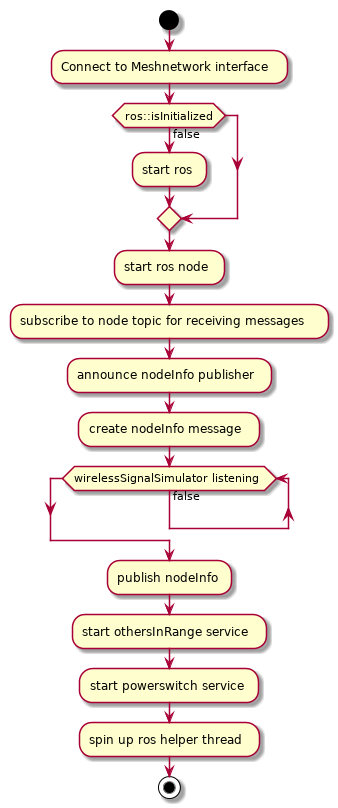
\includegraphics[width=.4\linewidth]{UML/out/ros/activity/StartAntenna/StartAntenna.png}\end{center}
	\caption{Activity diagram initialiseren van de DroneEngine}
	\label{fig:ros:MeshNetwerk:Activity:antenne}
\end{figure}

Als een antenne start legt die als eerste verbinding met zijn vereiste interface \nameref{architectural:interfaces:IMeshNetwork}. 
Vervolgens controleert de antenne of ros al draait als dit nog niet zo is start hij deze op.
Hierna start de antenne een rosnode op die hij gebruikt voor ros transport.
Zodra deze node opgestart is start de antenne met luisteren naar zijn eigen topic
Als dit topic aangemaakt is maakt hij een ros publisher aan voor de nodeInfo.  
Als dit gedaan is wacht de antenne tot de wirelessSignalSimulator luistert naar het topic.
Wanneer deze luistert publiceert de antenne de informatie.
Vervolgens worden de services opgestart om nodes binnen bereik te vinden en de powerswitch.
Tenslotte wordt er een thread opgestart voor het bufferen van ros berichten.

\subsection{Ontwerpkeuzes gemaakt voor het ros component}
\label{DetailedDesign:ros:ontwerkeuzes}
In het volgende stuk worden de keuzes gemaakt voor het component toegelicht.

\section{Design Sub-System NRF24}
\label{DetailedDesign:NRF24}

\subsection{Component Diagram}
\label{DetailedDesign:NRF24:ComponentDiagram}
\begin{figure}[H]
	\begin{center}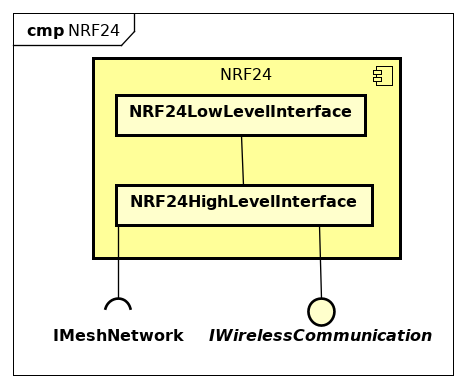
\includegraphics[width=.5\linewidth]{Afbeeldingen/NRF24ComponentDiagram.png}\end{center}
	\caption{component diagram ros}
	\label{fig:component:NRF24}
\end{figure}

Het component diagram bestaat uit twee interfaces. Een high level interface en een low level interface ook wel de driver genoemd.
De high level interface biedt de interface IWirelessCommunication aan. Omdat deze al volledig behandeld is in \autoref{DetailedDesign:ros:extern:interfaces:IWirelessCommunication} \nameref{DetailedDesign:ros:extern:interfaces:IWirelessCommunication} wordt deze niet nogmaals behandeld

\subsection{Aansluiting NRF24}

\begin{figure}[H]
	\begin{center}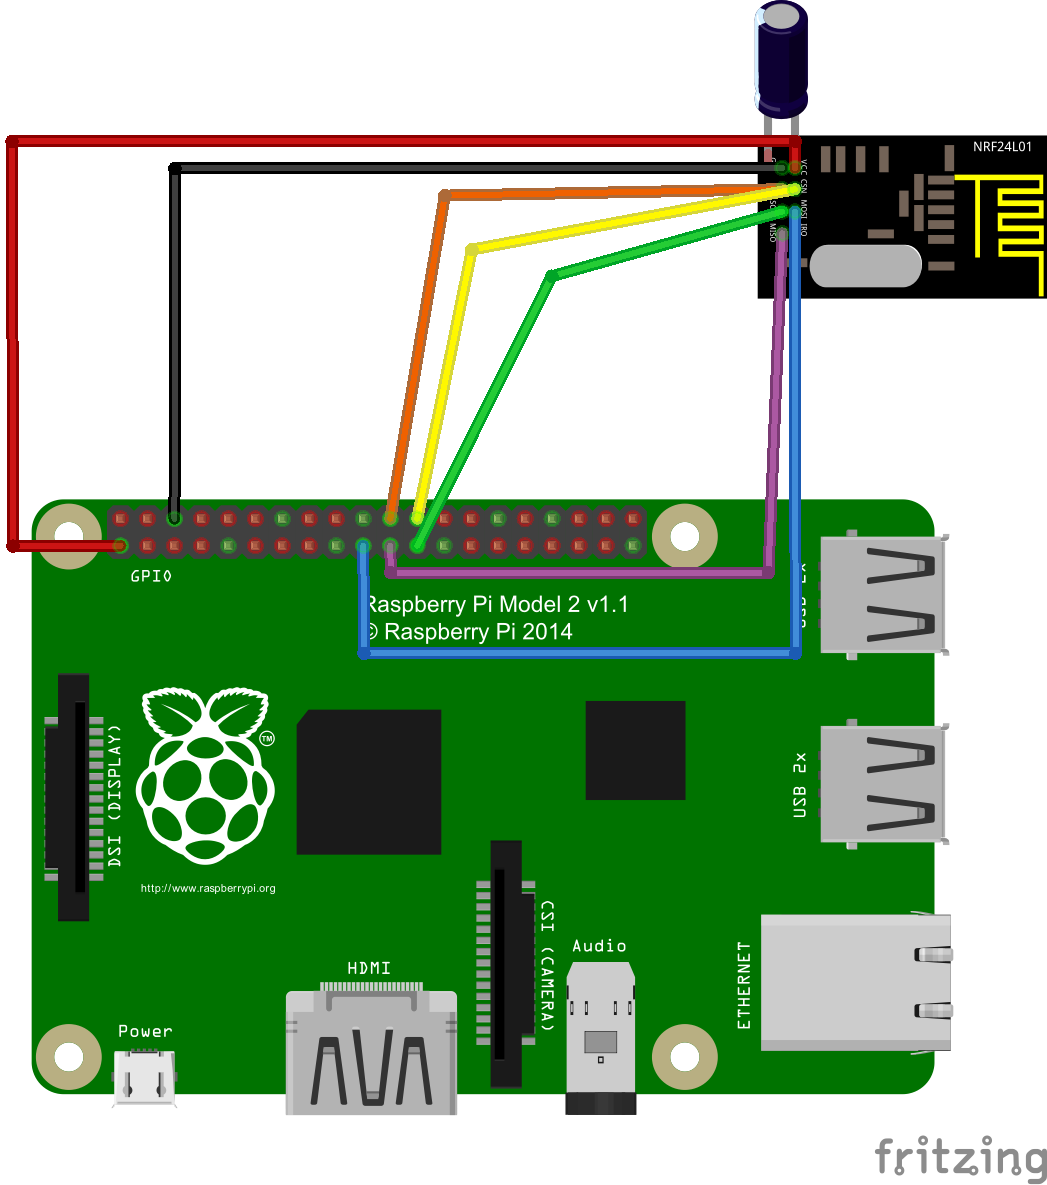
\includegraphics[width=.5\linewidth]{Afbeeldingen/fritzing_raspberry_nrf.png}\end{center}
	\caption{Aansluiting nRF24 op een Raspberry Pi}
	\label{fig:component:aansluting}
\end{figure}

Voor een stabieler voltage wordt een condensator van \SI{4.7}{\micro\farad} aanbevolen direct aangesloten op de ground en voltage poort van de nRF

\begin{table}[H]
	\centering
		\begin{tabular}{|l|c|r|}
			\hline
			\rowcolor[HTML]{C0C0C0} 
			Raspberry Pi & NRF24L01+ & Kleur \\ \hline
			6 / GND & GND & Zwart \\ \hline
			1 / 3.3V DC & VCC & Rood \\ \hline
			22 / GPIO25 & CE & Oranje \\ \hline
			24 / GPIO 8 & CSN/CS & Geel \\ \hline
			23 / GPIO11 / SPI\_CLK & SCK & Groen \\ \hline
			19 / GPIO10 / SPI\_MOSI & MOSI & Blauw \\ \hline
			21 / GPIO9 / SPI\_MISO & MISO & Paars \\ \hline
		\end{tabular}%
	\caption{Aansluitingen NRF24l01+ op een Raspberry Pi model 2B+}
	\label{tab:raspberry-nrf-aanslutingen}
\end{table}

\subsection{Sequence Diagrams}
\label{DetailedDesign:NRF24:sequence}

\paragraph{SetupNRF24}
\label{DetailedDesign:NRF24:sequence:SetupNRF24}

\begin{figure}[H]
	\begin{center}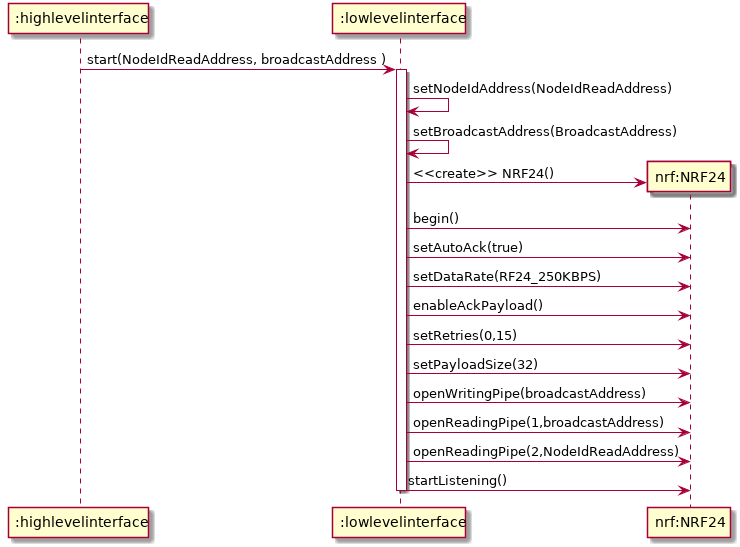
\includegraphics[width=1\linewidth]{UML/out/NRF24/sequence/SetupNRF24/SetupNRF24.png}\end{center}
	\caption{component diagram ros}
	\label{fig:NRF24:sequence:SetupNRF24}
\end{figure}


\paragraph{highlevelBroadcastMessage}
\label{DetailedDesign:NRF24:sequence:highlevelBroadcastMessage}

\begin{figure}[H]
	\begin{center}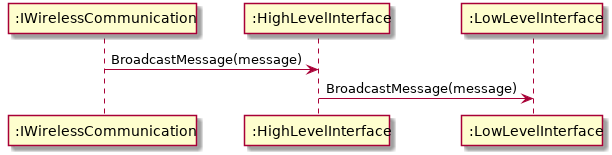
\includegraphics[width=1\linewidth]{UML/out/NRF24/sequence/highlevelBroadcastMessage/highlevelBroadcastMessage.png}\end{center}
	\caption{component diagram ros}
	\label{fig:NRF24:sequence:highlevelBroadcastMessage}
\end{figure}

\paragraph{highlevelSendMessage}
\label{DetailedDesign:NRF24:sequence:highlevelSendMessage}

\begin{figure}[H]
	\begin{center}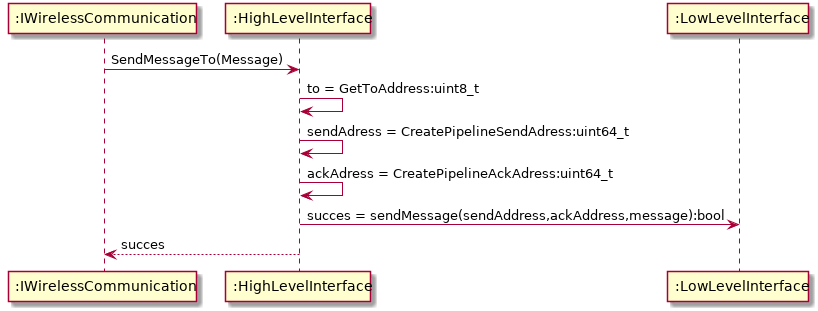
\includegraphics[width=1\linewidth]{UML/out/NRF24/sequence/highlevelSendMessage/highlevelSendMessage.png}\end{center}
	\caption{component diagram ros}
	\label{fig:NRF24:sequence:highlevelSendMessage}
\end{figure}

\paragraph{lowlevelBroadcastMessage}
\label{DetailedDesign:NRF24:sequence:lowlevelBroadcastMessage}

\begin{figure}[H]
	\begin{center}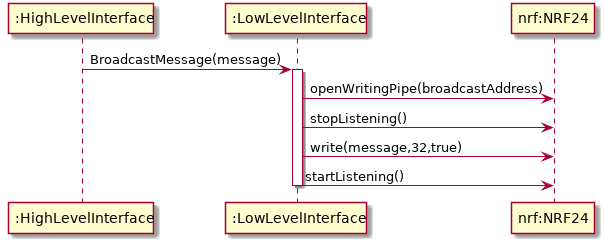
\includegraphics[width=1\linewidth]{UML/out/NRF24/sequence/lowlevelBroadcastMessage/lowlevelBroadcastMessage.png}\end{center}
	\caption{component diagram ros}
	\label{fig:NRF24:sequence:lowlevelBroadcastMessage}
\end{figure}

\paragraph{lowlevelSendMessage}
\label{DetailedDesign:NRF24:sequence:lowlevelSendMessage}

\begin{figure}[H]
	\begin{center}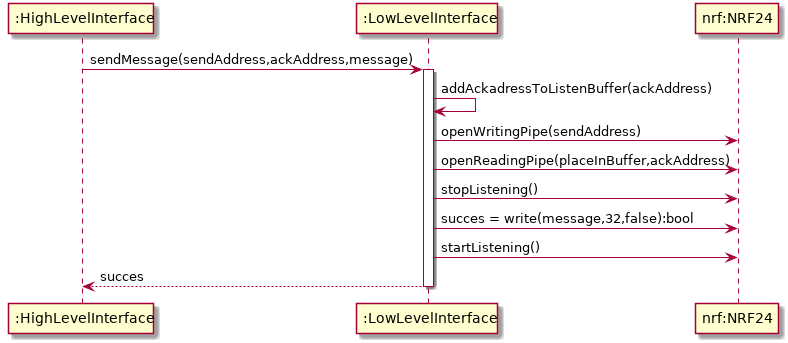
\includegraphics[width=1\linewidth]{UML/out/NRF24/sequence/lowlevelSendMessage/lowlevelSendMessage.png}\end{center}
	\caption{component diagram ros}
	\label{fig:NRF24:sequence:lowlevelSendMessage}
\end{figure}

\paragraph{recieveMessage}
\label{DetailedDesign:NRF24:sequence:recieveMessage}

\begin{figure}[H]
	\begin{center}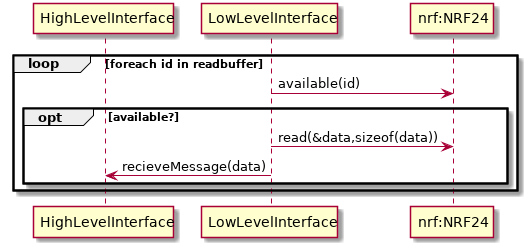
\includegraphics[width=1\linewidth]{UML/out/NRF24/sequence/recieveMessage/recieveMessage.png}\end{center}
	\caption{component diagram ros}
	\label{fig:NRF24:sequence:recieveMessage}
\end{figure}


\subsection{Activity Diagrams}
\label{DetailedDesign:NRF24:activity}

\paragraph{sendMessage}
\label{DetailedDesign:NRF24:activity:recieveMessage}

\begin{figure}[H]
	\begin{center}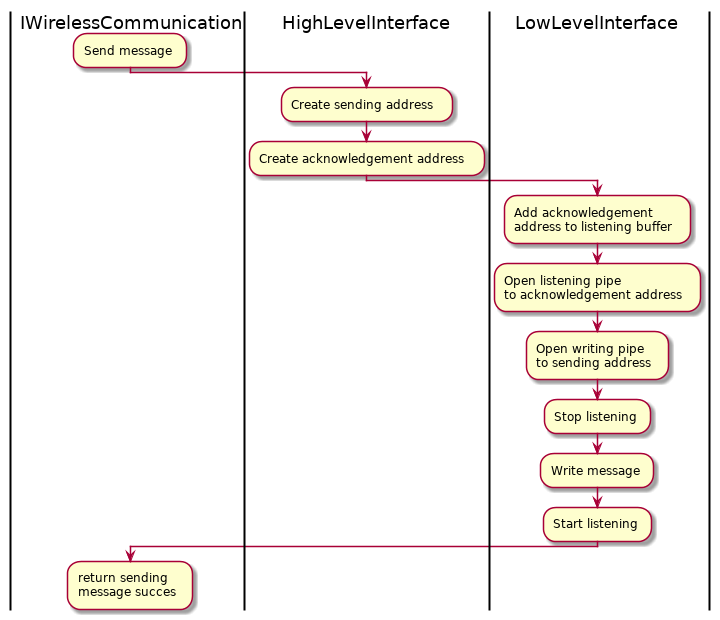
\includegraphics[width=1\linewidth]{UML/out/NRF24/activity/sendMessage/sendMessage.png}\end{center}
	\caption{component diagram ros}
	\label{fig:NRF24:activity:sendMessage}
\end{figure}

\paragraph{setupAntenna}
\label{DetailedDesign:NRF24:activity:setupAntenna}

\begin{figure}[H]
	\begin{center}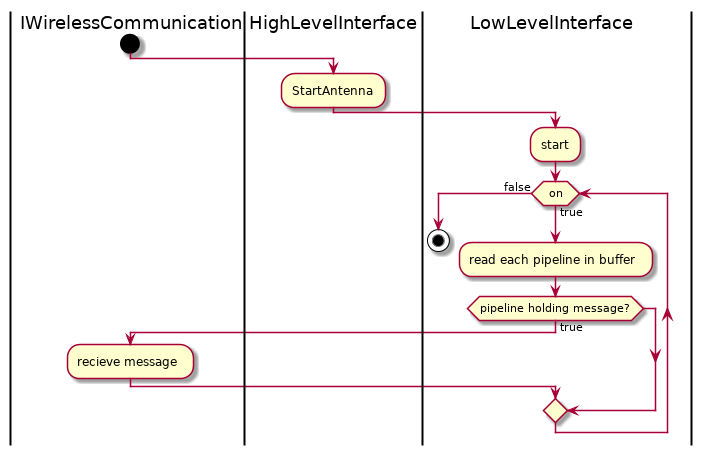
\includegraphics[width=1\linewidth]{UML/out/NRF24/activity/setupAntenna/setupAntenna.png}\end{center}
	\caption{component diagram ros}
	\label{fig:NRF24:activity:setupAntenna}
\end{figure}


\subsection{Ontwerpkeuzes gemaakt voor het NRF24 component}
\label{DetailedDesign:NRF24:ontwerkeuzes}
In het volgende stuk worden de keuzes gemaakt voor het component toegelicht.


\bibliographystyle{apacite}
\bibliography{bilbliography.bib}

\clearpage
\appendix
%\chapter{Appendix 1}
%\label{app:iteratieplan}





\end{document}